\chapter{RBFNN-based identification on an example network}
\label{NN_based_example}

\emph{In this part, the test results of the chosen identification method are presented on a simple EPANET example. }

\section{The network in EPANET}
\label{example1_EPANET}

A simple test network in EPANET has been used for testing the presented identification method. On a real world network, typically the control cannot be taken to its extremes, as this would result in undesired service to the customers. Therefore, the network shown in \figref{fig:epanet_example1_id} has been created to mimic the behaviour of a multi-inlet, single-WT system, such that the identification method, presented in \chapref{identification_design}, can be be tested under different operations. 

%EPANET example network for identification
\begin{figure}[H]
\centering
%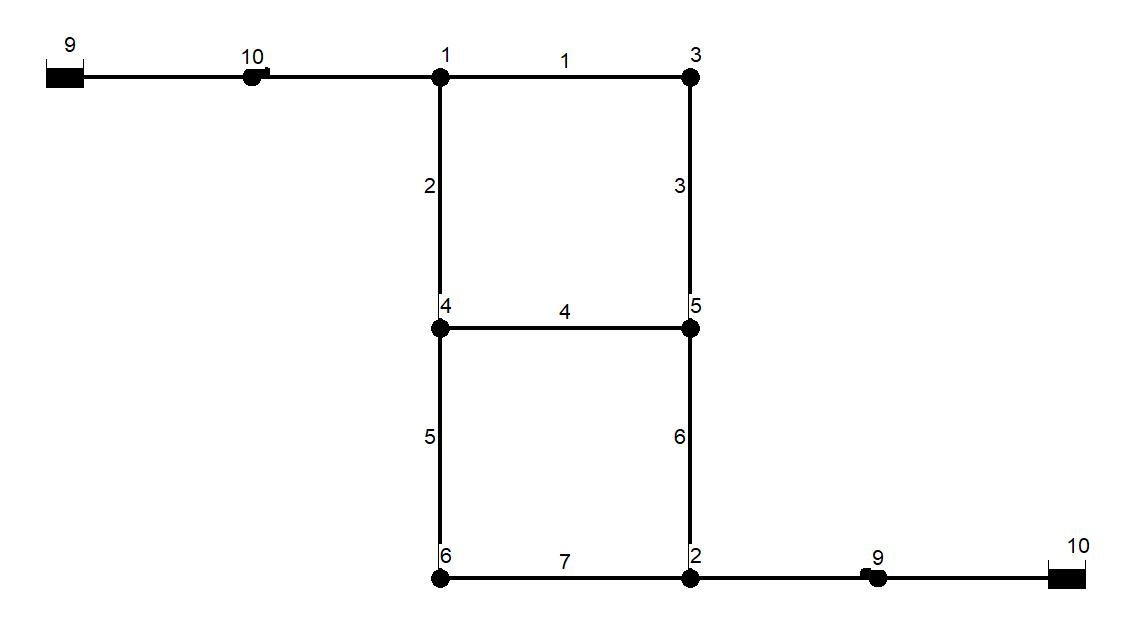
\includegraphics[width=0.6\textwidth]{report/pictures/example1_epanetmodel}
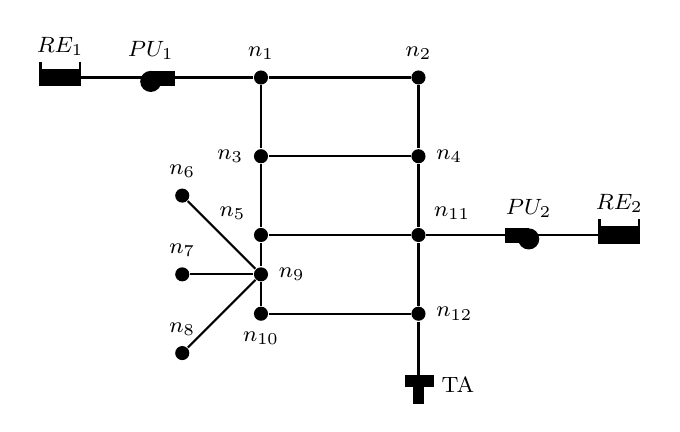
\begin{tikzpicture}[semithick,state/.style ={ draw,shape=circle,scale=0.9}]

\node[circle,fill,inner sep=1.8pt,label=above : \footnotesize$n_1$] (A) at (0,0) {};
\node[circle,fill,inner sep=1.8pt,label=above : \footnotesize$n_2$] (B) at (2,0) {};
\node[circle,fill,inner sep=1.8pt,label= left: \footnotesize$n_3$] (C) at (0,-1) {};
\node[circle,fill,inner sep=1.8pt,label= right: \footnotesize$n_4$] (D) at (2,-1) {};
\node[circle,fill,inner sep=1.8pt,label= above right: \footnotesize $n_{11}$] (E) at (2,-2) {};
\node[circle,fill,inner sep=1.8pt,label= above left: \footnotesize$n_5$] (F) at (0,-2) {};
\node[circle,fill,inner sep=1.8pt,label= below : \footnotesize$n_{10}$] (G) at (0,-3) {};
\node[circle,fill,inner sep=1.8pt,label=  right: \footnotesize$n_9$] (H) at (0,-2.5) {};
\node[circle,fill,inner sep=1.8pt,label=  right: \footnotesize$n_{12}$] (I) at (2,-3) {};
\node[circle,fill,inner sep=1.8pt,label=  above: \footnotesize$n_6$] (J) at (-1,-1.5) {};
\node[circle,fill,inner sep=1.8pt,label=  above: \footnotesize $n_7$] (M) at (-1,-2.5) {};
\node[circle,fill,inner sep=1.8pt,label=  above: \footnotesize $n_8$] (L) at (-1,-3.5) {};



\draw [thick] (A) --  (B) node[above  =0.05 cm] {\footnotesize$$};
\path (A) edge [thick]  node[left  =0.05 cm] {\footnotesize$$} (C);
\path (B) edge [thick] node[right  =0.05 cm] {\footnotesize$$} (D);
\path (C) edge [thick] node[above  =0.05 cm] {\footnotesize$$} (D);
\path (C) edge [thick] node[left  =0.05 cm] {\footnotesize$$} (F);
\path (D) edge [thick] node[right  =0.05 cm] {\footnotesize$$} (E);
\path (E) edge [thick] node[below  =0.05 cm] {\footnotesize$$} (F);
\path (F) edge [thick] node[below  =0.05 cm] {\footnotesize$$} (H);
\path (H) edge [thick] node[below  =0.05 cm] {\footnotesize$$} (G);
\path (H) edge [thick] node[below  =0.05 cm] {\footnotesize$$} (J);
\path (H) edge [thick] node[below  =0.05 cm] {\footnotesize$$} (M);
\path (H) edge [thick] node[below  =0.05 cm] {\footnotesize$$} (L);
\path (G) edge [thick] node[below  =0.05 cm] {\footnotesize$$} (I);
\path (E) edge [thick] node[below  =0.05 cm] {\footnotesize$$} (I);

%PU2
\node[circle,fill,inner sep=2.7pt,label= above : \footnotesize $ PU_2$] (I) at (3.4,-2.05) {};
\draw [thin,fill] (3.1,-1.92) rectangle (3.4,-2.1);


\begin{scope}[xscale=-1,yscale=1]
%PU1
\node[circle,fill,inner sep=2.7pt,label= above : \footnotesize $ PU_1$] (I) at (3.4-2,-2.05+2) {};
\draw [thin,fill] (3.1-2,-1.92+2) rectangle (3.4-2,-2.1+2);

\end{scope}

\draw [thick](2.1,-2) -- (3.1,-2);
\draw [thick, fill] (1.84,-3.79) rectangle (2.18,-3.92);
\draw [thick,fill] (1.95,-3.92) rectangle (2.06,-4.13);
\draw [thick](2,-3.1) -- (2,-3.8);
\node at (2.5,-3.9) {\footnotesize TA};


\draw [thick](-0.1,0) -- (-1.1,0);


\draw [thick](3.5,-2) -- (4.3,-2);
\draw [thick](-1.5,0) -- (-2.3,0);
\draw [thick](-2.3,0.2) -- (-2.3,-0.1) -- (-2.8,-0.1) -- (-2.8,0.2);
\draw [thick,fill] (-2.8,0.1) rectangle (-2.3,-0.1);
\draw [thick](4.3,-1.8) -- (4.3,-2.1) -- (4.8,-2.1) -- (4.8,-1.8);
\draw [thick,fill] (4.3,-1.9) rectangle (4.8,-2.1);
\node at (-2.55,0.4) {\footnotesize $RE_1$};
\node at (4.55,-1.6) {\footnotesize $RE_2$};
\end{tikzpicture} 
\caption{Multi-inlet, Single-WT example network.}
\label{fig:epanet_example1_id}
\end{figure}
\vspace{-3mm}

The network shown in \figref{fig:epanet_example1_id} consists of two pumping stations $PU_1$, $PU_2$ and a Water Tank $TA$. It should be noted that reservoirs $RE_1$ and $RE_2$ are required for simulating the pumps, however they differ from WTs in the sense that they cannot be emptied in the simulation. It is important to note that the physical parameters and numerical values do not represent any existing physical network, therefore quantitatively the values might be unrealistic compared to real world scenarios. The physical and operational properties of the test system can be found in \appref{physical_properties_example1}.

The controls implemented on the network are based on simple time scheduling of the two pumping stations. Both pumps turn off when the pressure head in the WT is above a certain limit. $PU_2$ turns on again if the pressure head in the WT decreases to some lower limit. Furthermore, $PU_2$ turns on again only if the pressure head provided by $PU_2$ exceeds some upper bound. 

\section{Identification and validation}
\label{identification_and_validation_of_the_output_eq} 

The identification is carried out on the simulation data, exported from EPANET. In order to validate the identified model, different control and consumption scenarios have been considered. Thus, in the first case of the validation, the model is tested by modifying the total consumption. In the second case, the consumption has been kept the same as for in the case of the identification, however the control properties of $PU_1$ and $PU_2$ has been modified. The two different consumption curves are both periodic with a time period of 24 hours and have the same characteristics. \figref{fig:sigma123} shows the $\sigma_1$ and $\sigma_2$ total consumption curves. 

  %Total consumptions
 \begin{figure}[H]
 \centering
 %\hspace{0mm}
 %
\includegraphics[width=0.35\textwidth]{report/pictures/missingfigure}
 % This file was created by matlab2tikz.
%
%The latest updates can be retrieved from
%  http://www.mathworks.com/matlabcentral/fileexchange/22022-matlab2tikz-matlab2tikz
%where you can also make suggestions and rate matlab2tikz.
%
\definecolor{mycolor1}{rgb}{0.00000,0.44700,0.74100}%
\definecolor{mycolor2}{rgb}{0.85000,0.32500,0.09800}%
\definecolor{mycolor3}{rgb}{0.92900,0.69400,0.12500}%
%
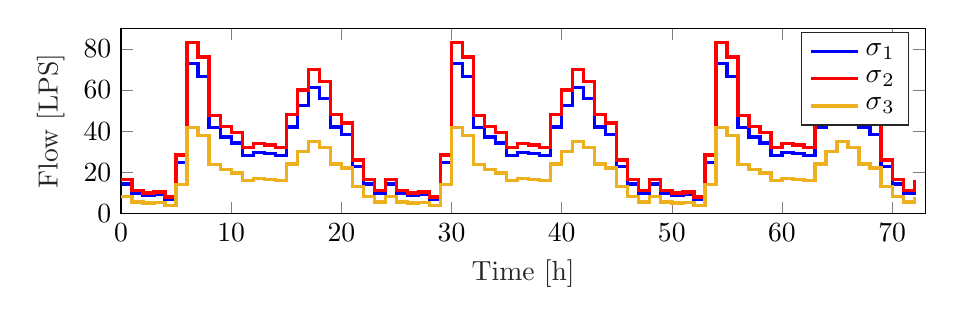
\begin{tikzpicture}

\begin{axis}[%
width=4.021in,
height=0.926in,
at={(0.758in,0.481in)},
scale only axis,
xmin=0,
xmax=73,
xlabel style={font=\color{white!15!black}},
xlabel={Time [h]},
ymin=0,
ymax=90,
ylabel style={font=\color{white!15!black}},
ylabel={Flow  [LPS]},
axis background/.style={fill=white},
legend style={legend cell align=left, align=left, draw=white!15!black}
]
\addplot[const plot, color=blue, line width=1.2pt] table[row sep=crcr] {%
0	14.35\\
1	9.8\\
2	8.75\\
3	9.1\\
4	7\\
5	24.85\\
6	72.8\\
7	66.5\\
8	41.65\\
9	37.1\\
10	34.3\\
11	28\\
12	29.75\\
13	29.05\\
14	28\\
15	42\\
16	52.5\\
17	61.25\\
18	56\\
19	42\\
20	38.5\\
21	22.75\\
22	14.35\\
23	9.8\\
24	14.35\\
25	9.8\\
26	8.75\\
27	9.1\\
28	7\\
29	24.85\\
30	72.8\\
31	66.5\\
32	41.65\\
33	37.1\\
34	34.3\\
35	28\\
36	29.75\\
37	29.05\\
38	28\\
39	42\\
40	52.5\\
41	61.25\\
42	56\\
43	42\\
44	38.5\\
45	22.75\\
46	14.35\\
47	9.8\\
48	14.35\\
49	9.8\\
50	8.75\\
51	9.1\\
52	7\\
53	24.85\\
54	72.8\\
55	66.5\\
56	41.65\\
57	37.1\\
58	34.3\\
59	28\\
60	29.75\\
61	29.05\\
62	28\\
63	42\\
64	52.5\\
65	61.25\\
66	56\\
67	42\\
68	38.5\\
69	22.75\\
70	14.35\\
71	9.8\\
72	14.35\\
};
\addlegendentry{$\sigma{}_\text{1}$}

\addplot[const plot, color=red, line width=1.2pt] table[row sep=crcr] {%
0	16.4\\
1	11.2\\
2	10\\
3	10.4\\
4	8\\
5	28.4\\
6	83.2\\
7	76\\
8	47.6\\
9	42.4\\
10	39.2\\
11	32\\
12	34\\
13	33.2\\
14	32\\
15	48\\
16	60\\
17	70\\
18	64\\
19	48\\
20	44\\
21	26\\
22	16.4\\
23	11.2\\
24	16.4\\
25	11.2\\
26	10\\
27	10.4\\
28	8\\
29	28.4\\
30	83.2\\
31	76\\
32	47.6\\
33	42.4\\
34	39.2\\
35	32\\
36	34\\
37	33.2\\
38	32\\
39	48\\
40	60\\
41	70\\
42	64\\
43	48\\
44	44\\
45	26\\
46	16.4\\
47	11.2\\
48	16.4\\
49	11.2\\
50	10\\
51	10.4\\
52	8\\
53	28.4\\
54	83.2\\
55	76\\
56	47.6\\
57	42.4\\
58	39.2\\
59	32\\
60	34\\
61	33.2\\
62	32\\
63	48\\
64	60\\
65	70\\
66	64\\
67	48\\
68	44\\
69	26\\
70	16.4\\
71	11.2\\
72	16.4\\
};
\addlegendentry{$\sigma{}_\text{2}$}

\addplot[const plot, color=mycolor3, line width=1.2pt] table[row sep=crcr] {%
0	8.2\\
1	5.6\\
2	5\\
3	5.2\\
4	4\\
5	14.2\\
6	41.6\\
7	38\\
8	23.8\\
9	21.2\\
10	19.6\\
11	16\\
12	17\\
13	16.6\\
14	16\\
15	24\\
16	30\\
17	35\\
18	32\\
19	24\\
20	22\\
21	13\\
22	8.2\\
23	5.6\\
24	8.2\\
25	5.6\\
26	5\\
27	5.2\\
28	4\\
29	14.2\\
30	41.6\\
31	38\\
32	23.8\\
33	21.2\\
34	19.6\\
35	16\\
36	17\\
37	16.6\\
38	16\\
39	24\\
40	30\\
41	35\\
42	32\\
43	24\\
44	22\\
45	13\\
46	8.2\\
47	5.6\\
48	8.2\\
49	5.6\\
50	5\\
51	5.2\\
52	4\\
53	14.2\\
54	41.6\\
55	38\\
56	23.8\\
57	21.2\\
58	19.6\\
59	16\\
60	17\\
61	16.6\\
62	16\\
63	24\\
64	30\\
65	35\\
66	32\\
67	24\\
68	22\\
69	13\\
70	8.2\\
71	5.6\\
72	8.2\\
};
\addlegendentry{$\sigma{}_\text{3}$}

\end{axis}
\end{tikzpicture}% 
 \vspace{-2.5mm}
 \caption{Consumption patterns used for identification and validation.}
 \label{fig:sigma123}
 \end{figure}

 \vspace{-3mm}

 \subsection{Identification}
 \label{identification}

 The identification has been carried out such that the total consumption in the network is $\sigma_1$. Furthermore, the control of the pumping stations is the following: both $PU_1$ and $PU_2$ shut down if the pressure head in the WT exceeds 19.85 meters. $PU_1$ turns on when the pressure head in the WT decreases to 19.55 meters and $PU_2$ turns on again only if the pressure head delivered by $PU_1$ is above 43 meters. The corresponding flow inputs $\bar{d}_{\mathcal{K}1}$, $\bar{d}_{\mathcal{K}2}$ and the pressure head in the WT $\hat{p}$ are shown in \figref{fig:identification_example1}.

 \vspace{-3mm}

   %Inlet flow - identification
 \begin{figure}[H]
 \centering
 %\hspace{0mm}
 %
\includegraphics[width=0.35\textwidth]{report/pictures/missingfigure}
 % This file was created by matlab2tikz.
%
%The latest updates can be retrieved from
%  http://www.mathworks.com/matlabcentral/fileexchange/22022-matlab2tikz-matlab2tikz
%where you can also make suggestions and rate matlab2tikz.
%
\definecolor{mycolor1}{rgb}{0.00000,0.44700,0.74100}%
\definecolor{mycolor2}{rgb}{0.85000,0.32500,0.09800}%
%
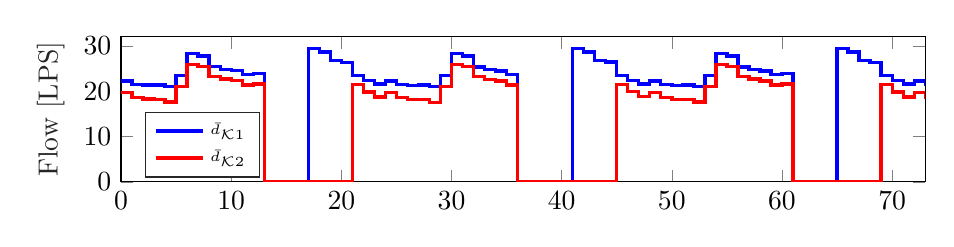
\begin{tikzpicture}

\begin{axis}[%
width=4.021in,
height=0.726in,
at={(0.75in,0.431in)},
scale only axis,
xmin=0,
xmax=73,
%xlabel style={font=\color{white!15!black}},
%xlabel={Time [h]},
ymin=0,
ymax=32,
ylabel style={font=\color{white!15!black}},
ylabel={Flow  [LPS]},
axis background/.style={fill=white},
legend style={at={(0.03,0.03)}, anchor=south west, legend cell align=left, align=left, draw=white!15!black}
]
\addplot[const plot, color=blue, line width=1.2pt] table[row sep=crcr] {%
0	22.26\\
1	21.53\\
2	21.33\\
3	21.35\\
4	20.98\\
5	23.44\\
6	28.3\\
7	27.77\\
8	25.37\\
9	24.83\\
10	24.49\\
11	23.74\\
12	23.92\\
13	0\\
14	0\\
15	0\\
16	0\\
17	29.39\\
18	28.62\\
19	26.75\\
20	26.38\\
21	23.49\\
22	22.31\\
23	21.57\\
24	22.24\\
25	21.51\\
26	21.31\\
27	21.33\\
28	20.96\\
29	23.41\\
30	28.28\\
31	27.75\\
32	25.34\\
33	24.81\\
34	24.47\\
35	23.72\\
36	0\\
37	0\\
38	0\\
39	0\\
40	0\\
41	29.41\\
42	28.64\\
43	26.77\\
44	26.4\\
45	23.5\\
46	22.32\\
47	21.59\\
48	22.25\\
49	21.52\\
50	21.32\\
51	21.34\\
52	20.97\\
53	23.43\\
54	28.29\\
55	27.77\\
56	25.36\\
57	24.83\\
58	24.48\\
59	23.73\\
60	23.91\\
61	0\\
62	0\\
63	0\\
64	0\\
65	29.4\\
66	28.62\\
67	26.76\\
68	26.38\\
69	23.49\\
70	22.31\\
71	21.58\\
72	22.24\\
73	21.51\\
74	21.31\\
75	21.33\\
76	20.96\\
77	23.42\\
78	28.28\\
79	27.75\\
80	25.35\\
81	24.81\\
82	24.47\\
83	23.72\\
84	0\\
85	0\\
86	0\\
87	0\\
88	0\\
89	29.41\\
90	28.63\\
91	26.77\\
92	26.39\\
93	23.5\\
94	22.32\\
95	21.59\\
96	22.25\\
97	21.52\\
98	21.32\\
99	21.34\\
100	20.97\\
101	23.43\\
102	28.29\\
103	27.76\\
104	25.36\\
105	24.82\\
106	24.48\\
107	23.73\\
108	0\\
109	0\\
110	0\\
111	0\\
112	0\\
113	29.4\\
114	28.63\\
115	26.76\\
116	26.38\\
117	23.49\\
118	22.31\\
119	21.58\\
120	22.24\\
121	21.51\\
122	21.31\\
123	21.33\\
124	20.96\\
125	23.42\\
126	28.28\\
127	27.76\\
128	25.35\\
129	24.82\\
130	24.47\\
131	23.72\\
132	0\\
133	0\\
134	0\\
135	0\\
136	0\\
137	29.41\\
138	28.63\\
139	26.77\\
140	26.39\\
141	23.5\\
142	22.32\\
143	21.59\\
144	22.25\\
145	21.52\\
146	21.32\\
147	21.34\\
};
\addlegendentry{\tiny $\bar{d}_{\mathcal{K}1}$}

\addplot[const plot, color=red, line width=1.2pt] table[row sep=crcr] {%
0	19.72\\
1	18.6\\
2	18.25\\
3	18.24\\
4	17.61\\
5	21.06\\
6	25.93\\
7	25.44\\
8	23.29\\
9	22.7\\
10	22.29\\
11	21.39\\
12	21.57\\
13	0\\
14	0\\
15	0\\
16	0\\
17	0\\
18	0\\
19	0\\
20	0\\
21	21.45\\
22	19.84\\
23	18.73\\
24	19.66\\
25	18.55\\
26	18.2\\
27	18.19\\
28	17.56\\
29	21\\
30	25.88\\
31	25.39\\
32	23.24\\
33	22.65\\
34	22.24\\
35	21.34\\
36	0\\
37	0\\
38	0\\
39	0\\
40	0\\
41	0\\
42	0\\
43	0\\
44	0\\
45	21.49\\
46	19.88\\
47	18.77\\
48	19.7\\
49	18.59\\
50	18.24\\
51	18.23\\
52	17.6\\
53	21.04\\
54	25.92\\
55	25.43\\
56	23.28\\
57	22.69\\
58	22.28\\
59	21.38\\
60	21.56\\
61	0\\
62	0\\
63	0\\
64	0\\
65	0\\
66	0\\
67	0\\
68	0\\
69	21.46\\
70	19.85\\
71	18.74\\
72	19.67\\
73	18.56\\
74	18.21\\
75	18.2\\
76	17.57\\
77	21.01\\
78	25.89\\
79	25.4\\
80	23.25\\
81	22.66\\
82	22.25\\
83	21.35\\
84	0\\
85	0\\
86	0\\
87	0\\
88	0\\
89	0\\
90	0\\
91	0\\
92	0\\
93	21.48\\
94	19.87\\
95	18.76\\
96	19.7\\
97	18.58\\
98	18.23\\
99	18.22\\
100	17.59\\
101	21.04\\
102	25.91\\
103	25.42\\
104	23.27\\
105	22.68\\
106	22.27\\
107	21.37\\
108	0\\
109	0\\
110	0\\
111	0\\
112	0\\
113	0\\
114	0\\
115	0\\
116	0\\
117	21.46\\
118	19.86\\
119	18.75\\
120	19.68\\
121	18.57\\
122	18.22\\
123	18.21\\
124	17.58\\
125	21.02\\
126	25.89\\
127	25.41\\
128	23.25\\
129	22.66\\
130	22.26\\
131	21.35\\
132	0\\
133	0\\
134	0\\
135	0\\
136	0\\
137	0\\
138	0\\
139	0\\
140	0\\
141	21.47\\
142	19.87\\
143	18.76\\
144	19.69\\
145	18.58\\
146	18.23\\
147	18.22\\
};
\addlegendentry{\tiny $\bar{d}_{\mathcal{K}2}$}

\end{axis}
\end{tikzpicture}% 
 \vspace{-2.5mm}
 %\caption{Inlet flows of $PU_1$ and $PU_2$.}
 \end{figure}

 \vspace{-5mm}

   %WT - identification
 \begin{figure}[H]
 \centering
 \hspace{-4.5mm}
 %
\includegraphics[width=0.35\textwidth]{report/pictures/missingfigure}
 % This file was created by matlab2tikz.
%
%The latest updates can be retrieved from
%  http://www.mathworks.com/matlabcentral/fileexchange/22022-matlab2tikz-matlab2tikz
%where you can also make suggestions and rate matlab2tikz.
%
\definecolor{mycolor1}{rgb}{0.00000,0.44700,0.74100}%
%
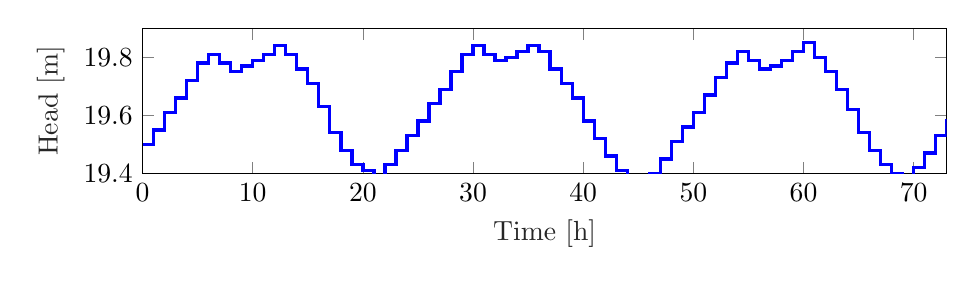
\begin{tikzpicture}

\begin{axis}[%
width=4.021in,
height=0.726in,
at={(0.792in,0.434in)},
scale only axis,
xmin=0,
xmax=73,
xlabel style={font=\color{white!15!black}},
xlabel={Time [h]},
ymin=19.4,
ymax=19.9,
ylabel style={font=\color{white!15!black}},
ylabel={Head  [m]},
axis background/.style={fill=white},
%legend style={legend cell align=left, align=left, draw=white!15!black}
]
\addplot[const plot, color=blue, line width=1.2pt, forget plot] table[row sep=crcr] {%
0	19.5\\
1	19.55\\
2	19.61\\
3	19.66\\
4	19.72\\
5	19.78\\
6	19.81\\
7	19.78\\
8	19.75\\
9	19.77\\
10	19.79\\
11	19.81\\
12	19.84\\
13	19.81\\
14	19.76\\
15	19.71\\
16	19.63\\
17	19.54\\
18	19.48\\
19	19.43\\
20	19.41\\
21	19.38\\
22	19.43\\
23	19.48\\
24	19.53\\
25	19.58\\
26	19.64\\
27	19.69\\
28	19.75\\
29	19.81\\
30	19.84\\
31	19.81\\
32	19.79\\
33	19.8\\
34	19.82\\
35	19.84\\
36	19.82\\
37	19.76\\
38	19.71\\
39	19.66\\
40	19.58\\
41	19.52\\
42	19.46\\
43	19.41\\
44	19.38\\
45	19.36\\
46	19.4\\
47	19.45\\
48	19.51\\
49	19.56\\
50	19.61\\
51	19.67\\
52	19.73\\
53	19.78\\
54	19.82\\
55	19.79\\
56	19.76\\
57	19.77\\
58	19.79\\
59	19.82\\
60	19.85\\
61	19.8\\
62	19.75\\
63	19.69\\
64	19.62\\
65	19.54\\
66	19.48\\
67	19.43\\
68	19.4\\
69	19.38\\
70	19.42\\
71	19.47\\
72	19.53\\
73	19.58\\
74	19.63\\
75	19.69\\
76	19.74\\
77	19.8\\
78	19.84\\
79	19.8\\
80	19.78\\
81	19.79\\
82	19.81\\
83	19.83\\
84	19.83\\
85	19.77\\
86	19.72\\
87	19.67\\
88	19.59\\
89	19.52\\
90	19.47\\
91	19.42\\
92	19.39\\
93	19.37\\
94	19.41\\
95	19.46\\
96	19.51\\
97	19.56\\
98	19.62\\
99	19.68\\
100	19.73\\
101	19.79\\
102	19.83\\
103	19.79\\
104	19.77\\
105	19.78\\
106	19.8\\
107	19.82\\
108	19.85\\
109	19.79\\
110	19.74\\
111	19.69\\
112	19.61\\
113	19.53\\
114	19.47\\
115	19.42\\
116	19.4\\
117	19.37\\
118	19.41\\
119	19.47\\
120	19.52\\
121	19.57\\
122	19.63\\
123	19.68\\
124	19.74\\
125	19.8\\
126	19.83\\
127	19.8\\
128	19.78\\
129	19.79\\
130	19.81\\
131	19.83\\
132	19.83\\
133	19.78\\
134	19.72\\
135	19.67\\
136	19.6\\
137	19.53\\
138	19.47\\
139	19.42\\
140	19.39\\
141	19.37\\
142	19.41\\
143	19.46\\
144	19.52\\
145	19.57\\
146	19.62\\
147	19.68\\
};
\end{axis}
\end{tikzpicture}% 
 \vspace{-2.5mm}
 \caption{Inlet flows(above) and the pressure in the WT(below) under $\sigma_1$ total demand.}
 \label{fig:identification_example1}
 \end{figure}

 \vspace{-3mm}


 \subsection{Validation 1}
 \label{validation_1}

 The first validation of the identified model has been carried out such that the total consumption is reduced to $\sigma_2$. The control properties are unchanged. The corresponding flow inputs $\bar{d}_{\mathcal{K}1}$, $\bar{d}_{\mathcal{K}2}$ and the pressure head in the WT $\hat{p}$ are shown in \figref{fig:identification_example1_v1}. 

 \vspace{-3mm}

   %Inlet flow - v1
 \begin{figure}[H]
 \centering
 %\hspace{0mm}
 %
\includegraphics[width=0.35\textwidth]{report/pictures/missingfigure}
 % This file was created by matlab2tikz.
%
%The latest updates can be retrieved from
%  http://www.mathworks.com/matlabcentral/fileexchange/22022-matlab2tikz-matlab2tikz
%where you can also make suggestions and rate matlab2tikz.
%
\definecolor{mycolor1}{rgb}{0.00000,0.44700,0.74100}%
\definecolor{mycolor2}{rgb}{0.85000,0.32500,0.09800}%
%
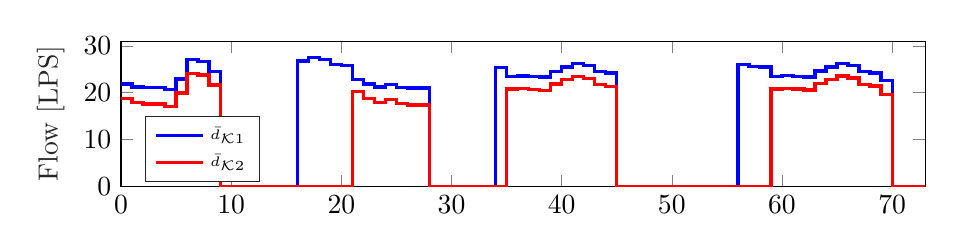
\begin{tikzpicture}

\begin{axis}[%
width=4.021in,
height=0.726in,
at={(0.75in,0.431in)},
scale only axis,
xmin=0,
xmax=73,
%xlabel style={font=\color{white!15!black}},
%xlabel={Time [h]},
ymin=0,
ymax=31,
ylabel style={font=\color{white!15!black}},
ylabel={Flow  [LPS]},
axis background/.style={fill=white},
legend style={at={(0.03,0.03)}, anchor=south west, legend cell align=left, align=left, draw=white!15!black}
]
\addplot[const plot, color=blue, line width=1.2pt] table[row sep=crcr] {%
0	21.83\\
1	21.22\\
2	21.04\\
3	21.05\\
4	20.74\\
5	22.89\\
6	27.02\\
7	26.59\\
8	24.46\\
9	0\\
10	0\\
11	0\\
12	0\\
13	0\\
14	0\\
15	0\\
16	26.73\\
17	27.52\\
18	27.07\\
19	26.02\\
20	25.79\\
21	22.88\\
22	21.82\\
23	21.21\\
24	21.75\\
25	21.14\\
26	20.97\\
27	20.97\\
28	0\\
29	0\\
30	0\\
31	0\\
32	0\\
33	0\\
34	25.43\\
35	23.41\\
36	23.56\\
37	23.46\\
38	23.32\\
39	24.57\\
40	25.48\\
41	26.22\\
42	25.77\\
43	24.52\\
44	24.2\\
45	0\\
46	0\\
47	0\\
48	0\\
49	0\\
50	0\\
51	0\\
52	0\\
53	0\\
54	0\\
55	0\\
56	25.95\\
57	25.64\\
58	25.46\\
59	23.43\\
60	23.59\\
61	23.48\\
62	23.34\\
63	24.6\\
64	25.51\\
65	26.25\\
66	25.79\\
67	24.54\\
68	24.22\\
69	22.63\\
70	0\\
71	0\\
72	0\\
73	0\\
74	0\\
75	0\\
76	0\\
77	0\\
78	0\\
79	0\\
80	25.93\\
81	25.63\\
82	25.45\\
83	23.42\\
84	23.58\\
85	23.47\\
86	23.33\\
87	24.59\\
88	25.5\\
89	26.24\\
90	25.78\\
91	24.53\\
92	24.22\\
93	22.62\\
94	0\\
95	0\\
96	0\\
97	0\\
98	0\\
99	0\\
100	0\\
101	0\\
102	0\\
103	0\\
104	25.94\\
105	25.64\\
106	25.45\\
107	23.42\\
108	23.58\\
109	23.48\\
110	23.33\\
111	24.59\\
112	25.5\\
113	26.24\\
114	25.79\\
115	24.53\\
116	24.22\\
117	22.62\\
118	0\\
119	0\\
120	0\\
121	0\\
122	0\\
123	0\\
124	0\\
125	0\\
126	0\\
127	0\\
128	25.94\\
129	25.64\\
130	25.45\\
131	23.42\\
132	23.58\\
133	23.48\\
134	23.33\\
135	24.59\\
136	25.5\\
137	26.24\\
138	25.79\\
139	24.53\\
140	24.22\\
141	22.62\\
142	0\\
143	0\\
144	0\\
145	0\\
146	0\\
147	0\\
};
\addlegendentry{\tiny $\bar{d}_{\mathcal{K}1}$}

\addplot[const plot, color=red, line width=1.2pt] table[row sep=crcr] {%
0	18.78\\
1	17.88\\
2	17.58\\
3	17.55\\
4	17.04\\
5	19.92\\
6	24.15\\
7	23.79\\
8	21.64\\
9	0\\
10	0\\
11	0\\
12	0\\
13	0\\
14	0\\
15	0\\
16	0\\
17	0\\
18	0\\
19	0\\
20	0\\
21	20.18\\
22	18.77\\
23	17.86\\
24	18.57\\
25	17.67\\
26	17.37\\
27	17.33\\
28	0\\
29	0\\
30	0\\
31	0\\
32	0\\
33	0\\
34	0\\
35	20.75\\
36	20.89\\
37	20.73\\
38	20.53\\
39	21.87\\
40	22.81\\
41	23.52\\
42	23.07\\
43	21.74\\
44	21.38\\
45	0\\
46	0\\
47	0\\
48	0\\
49	0\\
50	0\\
51	0\\
52	0\\
53	0\\
54	0\\
55	0\\
56	0\\
57	0\\
58	0\\
59	20.8\\
60	20.95\\
61	20.79\\
62	20.58\\
63	21.93\\
64	22.86\\
65	23.58\\
66	23.12\\
67	21.8\\
68	21.44\\
69	19.55\\
70	0\\
71	0\\
72	0\\
73	0\\
74	0\\
75	0\\
76	0\\
77	0\\
78	0\\
79	0\\
80	0\\
81	0\\
82	0\\
83	20.78\\
84	20.93\\
85	20.77\\
86	20.56\\
87	21.91\\
88	22.84\\
89	23.56\\
90	23.1\\
91	21.77\\
92	21.41\\
93	19.53\\
94	0\\
95	0\\
96	0\\
97	0\\
98	0\\
99	0\\
100	0\\
101	0\\
102	0\\
103	0\\
104	0\\
105	0\\
106	0\\
107	20.79\\
108	20.93\\
109	20.77\\
110	20.57\\
111	21.91\\
112	22.84\\
113	23.56\\
114	23.11\\
115	21.78\\
116	21.42\\
117	19.53\\
118	0\\
119	0\\
120	0\\
121	0\\
122	0\\
123	0\\
124	0\\
125	0\\
126	0\\
127	0\\
128	0\\
129	0\\
130	0\\
131	20.78\\
132	20.93\\
133	20.77\\
134	20.57\\
135	21.91\\
136	22.84\\
137	23.56\\
138	23.1\\
139	21.78\\
140	21.42\\
141	19.53\\
142	0\\
143	0\\
144	0\\
145	0\\
146	0\\
147	0\\
};
\addlegendentry{\tiny $\bar{d}_{\mathcal{K}2}$}

\end{axis}
\end{tikzpicture}% 
 \vspace{-2.5mm}
 %\caption{Inlet flows of $PU_1$ and $PU_2$.}
 \end{figure}

 \vspace{-5.5mm}

   %WT - sigma1
 \begin{figure}[H]
 \centering
 \hspace{-4.5mm}
 %
\includegraphics[width=0.35\textwidth]{report/pictures/missingfigure}
 % This file was created by matlab2tikz.
%
%The latest updates can be retrieved from
%  http://www.mathworks.com/matlabcentral/fileexchange/22022-matlab2tikz-matlab2tikz
%where you can also make suggestions and rate matlab2tikz.
%
\definecolor{mycolor1}{rgb}{0.00000,0.44700,0.74100}%
%
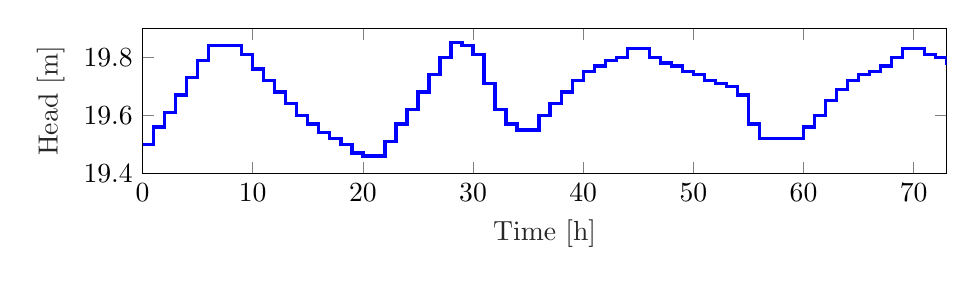
\begin{tikzpicture}

\begin{axis}[%
width=4.021in,
height=0.726in,
at={(0.792in,0.434in)},
scale only axis,
xmin=0,
xmax=73,
xlabel style={font=\color{white!15!black}},
xlabel={Time [h]},
ymin=19.4,
ymax=19.9,
ylabel style={font=\color{white!15!black}},
ylabel={Head  [m]},
axis background/.style={fill=white},
legend style={legend cell align=left, align=left, draw=white!15!black}
]
\addplot[const plot, color=blue, line width=1.2pt, forget plot] table[row sep=crcr] {%
0	19.5\\
1	19.56\\
2	19.61\\
3	19.67\\
4	19.73\\
5	19.79\\
6	19.84\\
7	19.84\\
8	19.84\\
9	19.81\\
10	19.76\\
11	19.72\\
12	19.68\\
13	19.64\\
14	19.6\\
15	19.57\\
16	19.54\\
17	19.52\\
18	19.5\\
19	19.47\\
20	19.46\\
21	19.46\\
22	19.51\\
23	19.57\\
24	19.62\\
25	19.68\\
26	19.74\\
27	19.8\\
28	19.85\\
29	19.84\\
30	19.81\\
31	19.71\\
32	19.62\\
33	19.57\\
34	19.55\\
35	19.55\\
36	19.6\\
37	19.64\\
38	19.68\\
39	19.72\\
40	19.75\\
41	19.77\\
42	19.79\\
43	19.8\\
44	19.83\\
45	19.83\\
46	19.8\\
47	19.78\\
48	19.77\\
49	19.75\\
50	19.74\\
51	19.72\\
52	19.71\\
53	19.7\\
54	19.67\\
55	19.57\\
56	19.52\\
57	19.52\\
58	19.52\\
59	19.52\\
60	19.56\\
61	19.6\\
62	19.65\\
63	19.69\\
64	19.72\\
65	19.74\\
66	19.75\\
67	19.77\\
68	19.8\\
69	19.83\\
70	19.83\\
71	19.81\\
72	19.8\\
73	19.78\\
74	19.77\\
75	19.76\\
76	19.74\\
77	19.74\\
78	19.7\\
79	19.61\\
80	19.54\\
81	19.53\\
82	19.53\\
83	19.53\\
84	19.58\\
85	19.62\\
86	19.66\\
87	19.7\\
88	19.74\\
89	19.75\\
90	19.77\\
91	19.78\\
92	19.81\\
93	19.85\\
94	19.82\\
95	19.8\\
96	19.79\\
97	19.77\\
98	19.76\\
99	19.75\\
100	19.74\\
101	19.73\\
102	19.69\\
103	19.6\\
104	19.53\\
105	19.53\\
106	19.53\\
107	19.53\\
108	19.57\\
109	19.61\\
110	19.66\\
111	19.7\\
112	19.73\\
113	19.75\\
114	19.76\\
115	19.78\\
116	19.81\\
117	19.84\\
118	19.83\\
119	19.81\\
120	19.79\\
121	19.77\\
122	19.76\\
123	19.75\\
124	19.74\\
125	19.73\\
126	19.7\\
127	19.6\\
128	19.54\\
129	19.53\\
130	19.53\\
131	19.53\\
132	19.57\\
133	19.62\\
134	19.66\\
135	19.7\\
136	19.73\\
137	19.75\\
138	19.76\\
139	19.78\\
140	19.81\\
141	19.84\\
142	19.82\\
143	19.81\\
144	19.79\\
145	19.77\\
146	19.76\\
147	19.75\\
};
\end{axis}
\end{tikzpicture}% 
 \vspace{-2.5mm}
 \caption{Inlet flows(above) and the pressure in the WT(below) under $\sigma_2$ total demand.}
 \label{fig:identification_example1_v1}
 \end{figure}

 \vspace{-3mm}

 As the consumer demand is reduced in the network, the pumping stations do not have to provide as much flow as in case of the identification. Therefore, the WT has a slower filling and emptying rate. 

 \subsection{Validation 2}
 \label{validation_2}

 In case of the second validation, the total consumption is $\sigma_1$, however the network is tested on different control properties. Thus, both $PU_1$ and $PU_2$ shut down if the pressure head in the WT exceeds 19.4 meters. $PU_1$ turns on when the pressure head in the WT decreases to 19.2 meters and $PU_2$ turns on again only if the pressure head delivered by $PU_1$ is above 48 meters. The corresponding flow inputs $\bar{d}_{\mathcal{K}1}$, $\bar{d}_{\mathcal{K}2}$ and the pressure head in the WT $\hat{p}$ are shown in \figref{fig:identification_example1_v2}.

 \vspace{-3mm}

   %Inlet flow - v2
 \begin{figure}[H]
 \centering
 %\hspace{0mm}
 %
\includegraphics[width=0.35\textwidth]{report/pictures/missingfigure}
 % This file was created by matlab2tikz.
%
%The latest updates can be retrieved from
%  http://www.mathworks.com/matlabcentral/fileexchange/22022-matlab2tikz-matlab2tikz
%where you can also make suggestions and rate matlab2tikz.
%
\definecolor{mycolor1}{rgb}{0.00000,0.44700,0.74100}%
\definecolor{mycolor2}{rgb}{0.85000,0.32500,0.09800}%
%
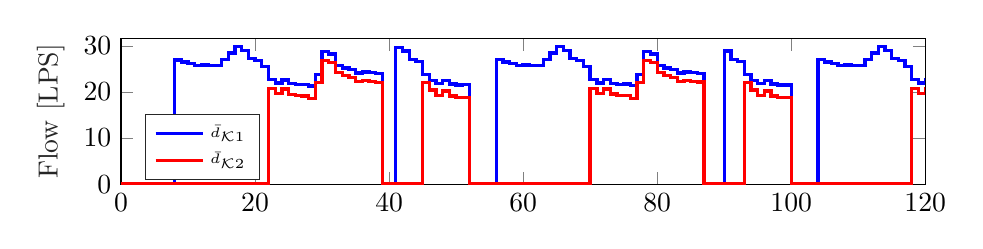
\begin{tikzpicture}

\begin{axis}[%
width=4.021in,
height=0.726in,
at={(0.75in,0.431in)},
scale only axis,
xmin=0,
xmax=120,
%xlabel style={font=\color{white!15!black}},
%xlabel={Time [h]},
ymin=0,
ymax=31.5,
ylabel style={font=\color{white!15!black}},
ylabel={Flow  [LPS]},
axis background/.style={fill=white},
legend style={at={(0.03,0.03)}, anchor=south west, legend cell align=left, align=left, draw=white!15!black}
]
\addplot[const plot, color=blue, line width=1.2pt] table[row sep=crcr] {%
0	0\\
1	0\\
2	0\\
3	0\\
4	0\\
5	0\\
6	0\\
7	0\\
8	26.95\\
9	26.47\\
10	26.21\\
11	25.67\\
12	25.83\\
13	25.77\\
14	25.69\\
15	27.06\\
16	28.45\\
17	29.81\\
18	29.04\\
19	27.21\\
20	26.84\\
21	25.46\\
22	22.68\\
23	21.94\\
24	22.61\\
25	21.87\\
26	21.66\\
27	21.68\\
28	21.31\\
29	23.82\\
30	28.73\\
31	28.2\\
32	25.75\\
33	25.21\\
34	24.86\\
35	24.11\\
36	24.29\\
37	24.18\\
38	24.04\\
39	0\\
40	0\\
41	29.66\\
42	28.89\\
43	27.04\\
44	26.67\\
45	23.73\\
46	22.53\\
47	21.79\\
48	22.46\\
49	21.72\\
50	21.52\\
51	21.54\\
52	0\\
53	0\\
54	0\\
55	0\\
56	26.96\\
57	26.48\\
58	26.22\\
59	25.69\\
60	25.84\\
61	25.79\\
62	25.7\\
63	27.07\\
64	28.46\\
65	29.82\\
66	29.05\\
67	27.22\\
68	26.85\\
69	25.48\\
70	22.69\\
71	21.95\\
72	22.62\\
73	21.88\\
74	21.67\\
75	21.69\\
76	21.32\\
77	23.83\\
78	28.74\\
79	28.21\\
80	25.76\\
81	25.22\\
82	24.87\\
83	24.12\\
84	24.3\\
85	24.19\\
86	24.05\\
87	0\\
88	0\\
89	0\\
90	28.88\\
91	27.03\\
92	26.66\\
93	23.72\\
94	22.52\\
95	21.78\\
96	22.45\\
97	21.72\\
98	21.51\\
99	21.53\\
100	0\\
101	0\\
102	0\\
103	0\\
104	26.96\\
105	26.48\\
106	26.22\\
107	25.69\\
108	25.84\\
109	25.79\\
110	25.7\\
111	27.07\\
112	28.46\\
113	29.82\\
114	29.05\\
115	27.22\\
116	26.85\\
117	25.48\\
118	22.69\\
119	21.95\\
120	22.62\\
121	21.88\\
122	21.67\\
123	21.69\\
124	21.32\\
125	23.84\\
126	28.75\\
127	28.21\\
128	25.76\\
129	25.22\\
130	24.87\\
131	24.13\\
132	24.3\\
133	24.19\\
134	24.06\\
135	0\\
136	0\\
137	0\\
138	28.88\\
139	27.03\\
140	26.66\\
141	23.72\\
142	22.52\\
143	21.78\\
144	22.45\\
145	21.71\\
146	21.51\\
147	21.53\\
};
\addlegendentry{\tiny $\bar{d}_{\mathcal{K}1}$}

\addplot[const plot, color=red, line width=1.2pt] table[row sep=crcr] {%
0	0\\
1	0\\
2	0\\
3	0\\
4	0\\
5	0\\
6	0\\
7	0\\
8	0\\
9	0\\
10	0\\
11	0\\
12	0\\
13	0\\
14	0\\
15	0\\
16	0\\
17	0\\
18	0\\
19	0\\
20	0\\
21	0\\
22	20.78\\
23	19.67\\
24	20.6\\
25	19.49\\
26	19.15\\
27	19.14\\
28	18.52\\
29	21.97\\
30	26.84\\
31	26.35\\
32	24.17\\
33	23.57\\
34	23.16\\
35	22.27\\
36	22.45\\
37	22.3\\
38	22.11\\
39	0\\
40	0\\
41	0\\
42	0\\
43	0\\
44	0\\
45	22.01\\
46	20.4\\
47	19.29\\
48	20.23\\
49	19.11\\
50	18.77\\
51	18.76\\
52	0\\
53	0\\
54	0\\
55	0\\
56	0\\
57	0\\
58	0\\
59	0\\
60	0\\
61	0\\
62	0\\
63	0\\
64	0\\
65	0\\
66	0\\
67	0\\
68	0\\
69	0\\
70	20.8\\
71	19.7\\
72	20.63\\
73	19.52\\
74	19.17\\
75	19.16\\
76	18.54\\
77	22\\
78	26.86\\
79	26.38\\
80	24.2\\
81	23.6\\
82	23.18\\
83	22.3\\
84	22.47\\
85	22.32\\
86	22.13\\
87	0\\
88	0\\
89	0\\
90	0\\
91	0\\
92	0\\
93	22\\
94	20.39\\
95	19.28\\
96	20.21\\
97	19.1\\
98	18.75\\
99	18.74\\
100	0\\
101	0\\
102	0\\
103	0\\
104	0\\
105	0\\
106	0\\
107	0\\
108	0\\
109	0\\
110	0\\
111	0\\
112	0\\
113	0\\
114	0\\
115	0\\
116	0\\
117	0\\
118	20.81\\
119	19.7\\
120	20.63\\
121	19.52\\
122	19.17\\
123	19.16\\
124	18.54\\
125	22\\
126	26.86\\
127	26.38\\
128	24.2\\
129	23.6\\
130	23.19\\
131	22.3\\
132	22.47\\
133	22.33\\
134	22.13\\
135	0\\
136	0\\
137	0\\
138	0\\
139	0\\
140	0\\
141	22\\
142	20.38\\
143	19.28\\
144	20.21\\
145	19.1\\
146	18.75\\
147	18.74\\
};
\addlegendentry{\tiny $\bar{d}_{\mathcal{K}2}$}

\end{axis}
\end{tikzpicture}% 
 \vspace{-2.5mm}
 %\caption{Inlet flows of $PU_1$ and $PU_2$.}
 \end{figure}

 \vspace{-5.5mm}

   %WT -v2
 \begin{figure}[H]
 \centering
 \hspace{-4.5mm}
 %
\includegraphics[width=0.35\textwidth]{report/pictures/missingfigure}
 % This file was created by matlab2tikz.
%
%The latest updates can be retrieved from
%  http://www.mathworks.com/matlabcentral/fileexchange/22022-matlab2tikz-matlab2tikz
%where you can also make suggestions and rate matlab2tikz.
%
\definecolor{mycolor1}{rgb}{0.00000,0.44700,0.74100}%
%
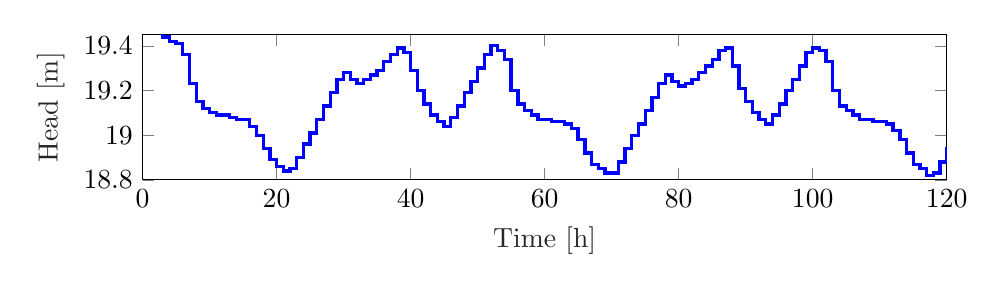
\begin{tikzpicture}

\begin{axis}[%
width=4.021in,
height=0.726in,
at={(0.792in,0.434in)},
scale only axis,
xmin=0,
xmax=120,
xlabel style={font=\color{white!15!black}},
xlabel={Time [h]},
ymin=18.8,
ymax=19.45,
ylabel style={font=\color{white!15!black}},
ylabel={Head  [m]},
axis background/.style={fill=white},
legend style={legend cell align=left, align=left, draw=white!15!black}
]
\addplot[const plot, color=blue, line width=1.2pt, forget plot] table[row sep=crcr] {%
0	19.5\\
1	19.47\\
2	19.46\\
3	19.44\\
4	19.42\\
5	19.41\\
6	19.36\\
7	19.23\\
8	19.15\\
9	19.12\\
10	19.1\\
11	19.09\\
12	19.09\\
13	19.08\\
14	19.07\\
15	19.07\\
16	19.04\\
17	19\\
18	18.94\\
19	18.89\\
20	18.86\\
21	18.84\\
22	18.85\\
23	18.9\\
24	18.96\\
25	19.01\\
26	19.07\\
27	19.13\\
28	19.19\\
29	19.25\\
30	19.28\\
31	19.25\\
32	19.23\\
33	19.25\\
34	19.27\\
35	19.29\\
36	19.33\\
37	19.36\\
38	19.39\\
39	19.37\\
40	19.29\\
41	19.2\\
42	19.14\\
43	19.09\\
44	19.06\\
45	19.04\\
46	19.08\\
47	19.13\\
48	19.19\\
49	19.24\\
50	19.3\\
51	19.36\\
52	19.4\\
53	19.38\\
54	19.34\\
55	19.2\\
56	19.14\\
57	19.11\\
58	19.09\\
59	19.07\\
60	19.07\\
61	19.06\\
62	19.06\\
63	19.05\\
64	19.03\\
65	18.98\\
66	18.92\\
67	18.87\\
68	18.85\\
69	18.83\\
70	18.83\\
71	18.88\\
72	18.94\\
73	19\\
74	19.05\\
75	19.11\\
76	19.17\\
77	19.23\\
78	19.27\\
79	19.24\\
80	19.22\\
81	19.23\\
82	19.25\\
83	19.28\\
84	19.31\\
85	19.34\\
86	19.38\\
87	19.39\\
88	19.31\\
89	19.21\\
90	19.15\\
91	19.1\\
92	19.07\\
93	19.05\\
94	19.09\\
95	19.14\\
96	19.2\\
97	19.25\\
98	19.31\\
99	19.37\\
100	19.39\\
101	19.38\\
102	19.33\\
103	19.2\\
104	19.13\\
105	19.11\\
106	19.09\\
107	19.07\\
108	19.07\\
109	19.06\\
110	19.06\\
111	19.05\\
112	19.02\\
113	18.98\\
114	18.92\\
115	18.87\\
116	18.85\\
117	18.82\\
118	18.83\\
119	18.88\\
120	18.94\\
121	18.99\\
122	19.05\\
123	19.11\\
124	19.17\\
125	19.23\\
126	19.27\\
127	19.24\\
128	19.21\\
129	19.23\\
130	19.25\\
131	19.28\\
132	19.31\\
133	19.34\\
134	19.37\\
135	19.39\\
136	19.31\\
137	19.22\\
138	19.15\\
139	19.1\\
140	19.07\\
141	19.05\\
142	19.09\\
143	19.15\\
144	19.2\\
145	19.26\\
146	19.31\\
147	19.37\\
};
\end{axis}
\end{tikzpicture}% 
 \vspace{-2.5mm}
 \caption{Inlet flows(above) and the pressure in the WT(below) under $\sigma_1$ total demand and under modified control properties.}
 \label{fig:identification_example1_v2}
 \end{figure}

 \vspace{-3mm}

 \subsection{Output model}
 \label{output model}

For the two inlet pressures $\bar{p}_{\mathcal{K}1}$ and $\bar{p}_{\mathcal{K}2}$, the identification has been carried out with six RBF neurons. The performance goal has been chosen to the order of $10^{-3}$. \figref{fig:MSE_output} shows the mean of squared errors in terms of RBF neurons. 

   %MSE output
 \begin{figure}[H]
 \centering
 %\hspace{0mm}
 %
\includegraphics[width=0.35\textwidth]{report/pictures/missingfigure}
 % This file was created by matlab2tikz.
%
%The latest updates can be retrieved from
%  http://www.mathworks.com/matlabcentral/fileexchange/22022-matlab2tikz-matlab2tikz
%where you can also make suggestions and rate matlab2tikz.
%
\definecolor{mycolor1}{rgb}{0.92900,0.69400,0.12500}%
\definecolor{mycolor2}{rgb}{0.49400,0.18400,0.55600}%
%
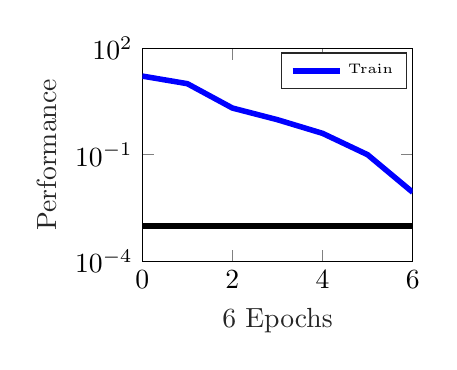
\begin{tikzpicture}

\begin{axis}[%
width=1.3521in,
height=1.066in,
at={(0.758in,0.481in)},
scale only axis,
xmin=0,
xmax=6,
xlabel style={font=\color{white!15!black}},
xlabel={6 Epochs},
ymode=log,
ymin=0.0001,
ymax=100,
yminorticks=true,
ylabel style={font=\color{white!15!black}},
ylabel={Performance},
axis background/.style={fill=white},
title style={},
%title={Performance is 0.00877771, Goal is 0.001},
legend style={legend cell align=left, align=left, draw=white!15!black}
]
\addplot [color=black, line width=2.0pt, forget plot]
  table[row sep=crcr]{%
0	0.001\\
1	0.001\\
2	0.001\\
3	0.001\\
4	0.001\\
5	0.001\\
6	0.001\\
};
\addplot [color=blue, line width=2.0pt]
  table[row sep=crcr]{%
0	16.3846300173484\\
1	10.0091945672363\\
2	2.0638352955794\\
3	0.968913605070296\\
4	0.400445250550717\\
5	0.100325503339624\\
6	0.00877770646781167\\
};
\addlegendentry{\tiny Train}

\addplot [color=mycolor1, forget plot]
  table[row sep=crcr]{%
0	0\\
};
\addplot [color=mycolor2, forget plot]
  table[row sep=crcr]{%
0	0\\
};
\end{axis}
\end{tikzpicture}% 
 \vspace{-2.5mm}
 \caption{The network’s performance according to the mean of squared errors.}
 \label{fig:MSE_output}
 \end{figure}

 \vspace{-4mm}

The performance goal can be reached with introducing more RBF neurons, however it does not generalize the model as well as six neurons. In case of increasing the number of neurons, and change the spread parameter of the RBFs, the identification has resulted in overfit and the validation has given bad performance. The identification of $\bar{p}_{\mathcal{K}1}$ and $\bar{p}_{\mathcal{K}2}$ inlet pressures in case of $\sigma_1$ total demand is shown in \figref{fig:pk_ident}. The two validations are shown in \figref{fig:pk_v1_ident}  and \figref{fig:pk_v2_ident}, respectively. 

   %pk1 - pk2 
 \begin{figure}[H]
 \centering
 %\hspace{-10mm}
 %
\includegraphics[width=0.35\textwidth]{report/pictures/missingfigure}
 % This file was created by matlab2tikz.
%
%The latest updates can be retrieved from
%  http://www.mathworks.com/matlabcentral/fileexchange/22022-matlab2tikz-matlab2tikz
%where you can also make suggestions and rate matlab2tikz.
%
\definecolor{mycolor1}{rgb}{0.00000,0.44700,0.74100}%
\definecolor{mycolor2}{rgb}{0.85000,0.32500,0.09800}%
%
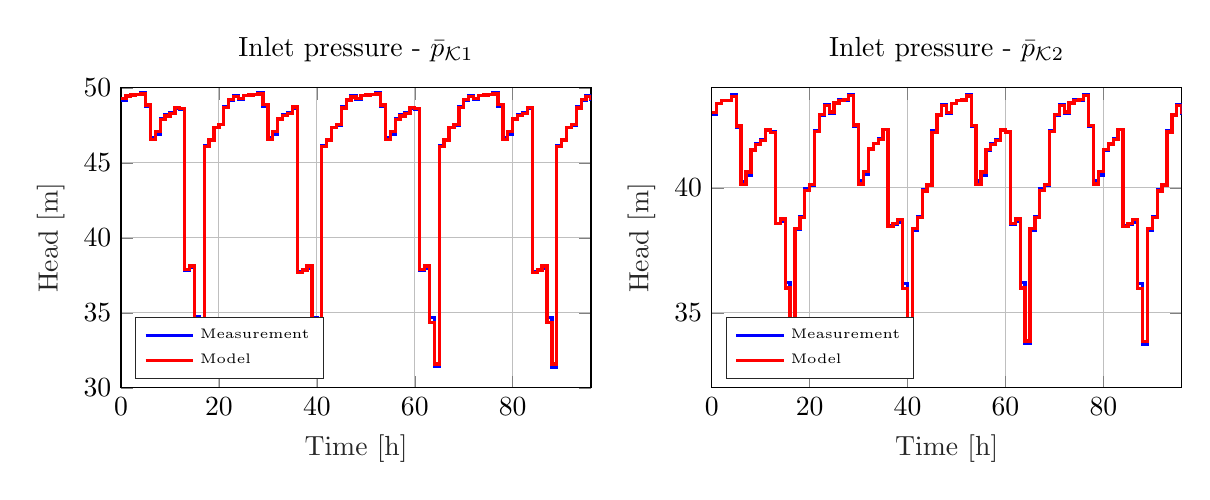
\begin{tikzpicture}

\begin{axis}[%
width=2.35in,
height=1.5in,
at={(1.232in,0.407in)},
scale only axis,
xmin=0,
xmax=96,
xlabel style={font=\color{white!15!black}},
xlabel={Time [h]},
ymin=30,
ymax=50,
grid,
ylabel style={font=\color{white!15!black}},
ylabel={Head  [m]},
axis background/.style={fill=white},
title style={},
title={Inlet pressure - $\bar{p}_{\mathcal{K}1}$},
legend style={at={(0.03,0.03)}, anchor=south west, legend cell align=left, align=left, draw=white!15!black}
]
\addplot[const plot, color=blue, line width=1.2pt] table[row sep=crcr] {%
0	49.2\\
1	49.47\\
2	49.54\\
3	49.54\\
4	49.67\\
5	48.76\\
6	46.66\\
7	46.91\\
8	47.97\\
9	48.19\\
10	48.34\\
11	48.64\\
12	48.57\\
13	37.86\\
14	38.01\\
15	34.72\\
16	31.43\\
17	46.13\\
18	46.51\\
19	47.37\\
20	47.54\\
21	48.74\\
22	49.19\\
23	49.45\\
24	49.21\\
25	49.48\\
26	49.55\\
27	49.54\\
28	49.67\\
29	48.77\\
30	46.67\\
31	46.92\\
32	47.98\\
33	48.2\\
34	48.35\\
35	48.65\\
36	37.72\\
37	37.81\\
38	37.96\\
39	34.67\\
40	31.38\\
41	46.12\\
42	46.5\\
43	47.36\\
44	47.53\\
45	48.73\\
46	49.18\\
47	49.45\\
48	49.21\\
49	49.47\\
50	49.55\\
51	49.54\\
52	49.67\\
53	48.76\\
54	46.66\\
55	46.91\\
56	47.97\\
57	48.2\\
58	48.34\\
59	48.64\\
60	48.57\\
61	37.85\\
62	37.99\\
63	34.7\\
64	31.42\\
65	46.13\\
66	46.51\\
67	47.37\\
68	47.53\\
69	48.74\\
70	49.18\\
71	49.45\\
72	49.21\\
73	49.48\\
74	49.55\\
75	49.54\\
76	49.67\\
77	48.76\\
78	46.67\\
79	46.92\\
80	47.98\\
81	48.2\\
82	48.34\\
83	48.64\\
84	37.73\\
85	37.82\\
86	37.97\\
87	34.68\\
88	31.39\\
89	46.13\\
90	46.5\\
91	47.36\\
92	47.53\\
93	48.73\\
94	49.18\\
95	49.45\\
96	49.21\\
97	49.47\\
98	49.55\\
99	49.54\\
100	49.67\\
101	48.76\\
102	46.66\\
103	46.91\\
104	47.98\\
105	48.2\\
106	48.34\\
107	48.64\\
108	37.75\\
109	37.84\\
110	37.99\\
111	34.69\\
112	31.41\\
113	46.13\\
114	46.5\\
115	47.37\\
116	47.53\\
117	48.73\\
118	49.18\\
119	49.45\\
120	49.21\\
121	49.48\\
122	49.55\\
123	49.54\\
124	49.67\\
125	48.76\\
126	46.67\\
127	46.91\\
128	47.98\\
129	48.2\\
130	48.34\\
131	48.64\\
132	37.74\\
133	37.82\\
134	37.97\\
135	34.68\\
136	31.39\\
137	46.13\\
138	46.5\\
139	47.36\\
140	47.53\\
141	48.73\\
142	49.18\\
143	49.45\\
144	49.21\\
145	49.48\\
146	49.55\\
147	49.54\\
};
\addlegendentry{\tiny Measurement}

\addplot[const plot, color=red, line width=1.2pt] table[row sep=crcr] {%
0	49.2729822630305\\
1	49.4637200766583\\
2	49.5150874766135\\
3	49.54500063276\\
4	49.581783927756\\
5	48.86138867298\\
6	46.5500534286232\\
7	47.0707002901576\\
8	47.9035931661685\\
9	48.1217282670262\\
10	48.2892129405389\\
11	48.6930561258448\\
12	48.605549098515\\
13	37.8739449785969\\
14	38.1313902354228\\
15	34.3595713274534\\
16	31.6009013887759\\
17	46.096215422368\\
18	46.5162831696101\\
19	47.3663605171029\\
20	47.5506090861633\\
21	48.6793785764258\\
22	49.2212035336494\\
23	49.4163747730986\\
24	49.2962904951694\\
25	49.4833341726267\\
26	49.5339826471921\\
27	49.5638904390536\\
28	49.5993330178279\\
29	48.8860275796541\\
30	46.5551776525447\\
31	47.0790171117227\\
32	47.9259868956415\\
33	48.1427758013849\\
34	48.310777464329\\
35	48.715321674492\\
36	37.6941402036515\\
37	37.8608587054011\\
38	38.1181681376068\\
39	34.3487646297874\\
40	31.5932032807154\\
41	46.0989882428669\\
42	46.5179449442707\\
43	47.3649356373936\\
44	47.5453578771222\\
45	48.6621213170306\\
46	49.201499604766\\
47	49.3977057641417\\
48	49.2809756672912\\
49	49.4696905373561\\
50	49.5169664966682\\
51	49.5507993022734\\
52	49.5872902507471\\
53	48.8655121719463\\
54	46.5500801761454\\
55	47.0737432597666\\
56	47.9084131232302\\
57	48.1239717151327\\
58	48.2909311531509\\
59	48.6990559373599\\
60	48.6114128107606\\
61	37.8713303366469\\
62	38.128748438709\\
63	34.3552522054816\\
64	31.5993639497355\\
65	46.0990141616274\\
66	46.5162831696101\\
67	47.3685057640532\\
68	47.5475666828994\\
69	48.6772432969546\\
70	49.21541341476\\
71	49.4103310658308\\
72	49.294680123615\\
73	49.4821024991388\\
74	49.5289392007893\\
75	49.5627701438557\\
76	49.5945973924013\\
77	48.8798471199545\\
78	46.5537369003986\\
79	47.0759856720664\\
80	47.9211883885645\\
81	48.1368245511267\\
82	48.304736654727\\
83	48.7092059381491\\
84	37.6967370041908\\
85	37.8634785712888\\
86	38.1208151785593\\
87	34.3509283397589\\
88	31.5947450836148\\
89	46.0989882428669\\
90	46.5171158796622\\
91	47.3677929562067\\
92	47.5464641619881\\
93	48.6684620420768\\
94	49.2073009978034\\
95	49.4029946024895\\
96	49.2809756672912\\
97	49.4709300837517\\
98	49.5220216366201\\
99	49.5558618764405\\
100	49.5881990210893\\
101	48.8696175460503\\
102	46.5522776712431\\
103	47.0733496968948\\
104	47.914134948774\\
105	48.1292839823936\\
106	48.2969824704023\\
107	48.7011389120493\\
108	37.701926694478\\
109	37.8687143876392\\
110	38.1261053298645\\
111	34.3552522054816\\
112	31.5978254187831\\
113	46.0976036333162\\
114	46.5171158796622\\
115	47.3656499503809\\
116	47.5475666828994\\
117	48.6730469792213\\
118	49.2096192071673\\
119	49.409049342315\\
120	49.2889528022068\\
121	49.4768894657902\\
122	49.527822181898\\
123	49.5577150316498\\
124	49.5936941131863\\
125	48.8778305178706\\
126	46.5529875802704\\
127	47.0763869031995\\
128	47.9211883885645\\
129	48.1374781100075\\
130	48.3025348828093\\
131	48.7092059381491\\
132	37.6967370041908\\
133	37.8660971322281\\
134	38.1208151785593\\
135	34.3509283397589\\
136	31.5962857965536\\
137	46.1004001976818\\
138	46.5171158796622\\
139	47.3677929562067\\
140	47.5464641619881\\
141	48.6706025123039\\
142	49.2073009978034\\
143	49.4029946024895\\
144	49.2867102202972\\
145	49.4749109690307\\
146	49.5220216366201\\
147	49.5558618764405\\
};
\addlegendentry{\tiny Model}

\end{axis}

\begin{axis}[%
xshift=-3.1cm,
width=2.35in,
height=1.5in,
at={(5.406in,0.407in)},
scale only axis,
xmin=0,
xmax=96,
grid,
xlabel style={font=\color{white!15!black}},
xlabel={Time [h]},
ymin=32,
ymax=44,
ylabel style={font=\color{white!15!black}},
ylabel={Head  [m]},
axis background/.style={fill=white},
title style={},
title={Inlet pressure - $\bar{p}_{\mathcal{K}2}$},
legend style={at={(0.03,0.03)}, anchor=south west, legend cell align=left, align=left, draw=white!15!black}
]
\addplot[const plot, color=blue, line width=1.2pt] table[row sep=crcr] {%
0	42.96\\
1	43.37\\
2	43.49\\
3	43.5\\
4	43.71\\
5	42.44\\
6	40.26\\
7	40.5\\
8	41.5\\
9	41.76\\
10	41.93\\
11	42.31\\
12	42.23\\
13	38.58\\
14	38.68\\
15	36.22\\
16	33.78\\
17	38.33\\
18	38.86\\
19	39.96\\
20	40.11\\
21	42.29\\
22	42.92\\
23	43.33\\
24	42.98\\
25	43.39\\
26	43.51\\
27	43.52\\
28	43.73\\
29	42.47\\
30	40.29\\
31	40.53\\
32	41.53\\
33	41.78\\
34	41.96\\
35	42.33\\
36	38.48\\
37	38.53\\
38	38.62\\
39	36.17\\
40	33.73\\
41	38.31\\
42	38.84\\
43	39.93\\
44	40.09\\
45	42.27\\
46	42.9\\
47	43.31\\
48	42.97\\
49	43.38\\
50	43.5\\
51	43.5\\
52	43.72\\
53	42.45\\
54	40.27\\
55	40.51\\
56	41.51\\
57	41.77\\
58	41.94\\
59	42.31\\
60	42.24\\
61	38.56\\
62	38.66\\
63	36.21\\
64	33.77\\
65	38.32\\
66	38.85\\
67	39.95\\
68	40.11\\
69	42.28\\
70	42.91\\
71	43.32\\
72	42.98\\
73	43.39\\
74	43.51\\
75	43.51\\
76	43.73\\
77	42.46\\
78	40.28\\
79	40.52\\
80	41.52\\
81	41.78\\
82	41.95\\
83	42.33\\
84	38.49\\
85	38.54\\
86	38.63\\
87	36.18\\
88	33.74\\
89	38.31\\
90	38.84\\
91	39.94\\
92	40.09\\
93	42.27\\
94	42.91\\
95	43.31\\
96	42.97\\
97	43.38\\
98	43.5\\
99	43.5\\
100	43.72\\
101	42.45\\
102	40.27\\
103	40.51\\
104	41.51\\
105	41.77\\
106	41.94\\
107	42.32\\
108	38.51\\
109	38.56\\
110	38.65\\
111	36.2\\
112	33.76\\
113	38.32\\
114	38.85\\
115	39.95\\
116	40.1\\
117	42.28\\
118	42.91\\
119	43.32\\
120	42.98\\
121	43.38\\
122	43.51\\
123	43.51\\
124	43.72\\
125	42.46\\
126	40.28\\
127	40.52\\
128	41.52\\
129	41.77\\
130	41.95\\
131	42.32\\
132	38.5\\
133	38.54\\
134	38.64\\
135	36.19\\
136	33.75\\
137	38.31\\
138	38.84\\
139	39.94\\
140	40.1\\
141	42.28\\
142	42.91\\
143	43.32\\
144	42.97\\
145	43.38\\
146	43.5\\
147	43.51\\
};
\addlegendentry{\tiny Measurement}

\addplot[const plot, color=red, line width=1.2pt] table[row sep=crcr] {%
0	43.0036018400701\\
1	43.3689734876142\\
2	43.4823944657657\\
3	43.5061923641111\\
4	43.6679262740055\\
5	42.4814419564929\\
6	40.1394950348589\\
7	40.6303576719845\\
8	41.5197823869906\\
9	41.7391835355291\\
10	41.9053102237853\\
11	42.3109284548824\\
12	42.2260083250224\\
13	38.587711993225\\
14	38.7587487473261\\
15	36.0004744727991\\
16	33.8754736113113\\
17	38.3857485440707\\
18	38.8283124705513\\
19	39.8849960143928\\
20	40.1303738632155\\
21	42.2478338520583\\
22	42.9386250772003\\
23	43.3080455621483\\
24	43.0320372291755\\
25	43.3949966558696\\
26	43.5079589273557\\
27	43.5317341132326\\
28	43.6926174904678\\
29	42.5118463531941\\
30	40.1533522509124\\
31	40.6464878834287\\
32	41.5509099447349\\
33	41.764912741389\\
34	41.9315155090718\\
35	42.3379060040743\\
36	38.4610278081728\\
37	38.5638622993522\\
38	38.7347980757011\\
39	35.978145070107\\
40	33.8551944898413\\
41	38.3779879506854\\
42	38.819696468664\\
43	39.8741426557234\\
44	40.113936943274\\
45	42.2285867177682\\
46	42.9144086808433\\
47	43.2827809296369\\
48	43.013774672421\\
49	43.3777041691571\\
50	43.4853763116029\\
51	43.5148045811909\\
52	43.6763387156312\\
53	42.4858540831117\\
54	40.1436661954868\\
55	40.635100252657\\
56	41.5275216564348\\
57	41.7405321293426\\
58	41.9080657302703\\
59	42.3195864258743\\
60	42.2345602281328\\
61	38.5829444142329\\
62	38.7539609805699\\
63	35.9915459902171\\
64	33.8714198304648\\
65	38.3858337130045\\
66	38.8283124705513\\
67	39.8844917688356\\
68	40.1253279029561\\
69	42.2464006985816\\
70	42.9316494956516\\
71	43.2992633507709\\
72	43.0308654232017\\
73	43.3940329041911\\
74	43.5014272310556\\
75	43.5308411109671\\
76	43.6862783125953\\
77	42.50304358173\\
78	40.1526854487942\\
79	40.6417538541293\\
80	41.5431854579146\\
81	41.7581014938821\\
82	41.9246190738943\\
83	42.3308939182761\\
84	38.4657825404758\\
85	38.5686345969735\\
86	38.7395905766369\\
87	35.9826131356873\\
88	33.8592523567361\\
89	38.3779879506854\\
90	38.82400572751\\
91	39.8790649313365\\
92	40.1196337467987\\
93	42.2358303344706\\
94	42.9213926324808\\
95	43.2894733008672\\
96	43.013774672421\\
97	43.378673657482\\
98	43.4919167145813\\
99	43.5213433948211\\
100	43.6771082244594\\
101	42.4915878058376\\
102	40.1478531827248\\
103	40.6360604637487\\
104	41.5341428819622\\
105	41.748647757271\\
106	41.9149699619912\\
107	42.3209166540963\\
108	38.4752884719391\\
109	38.5781756549033\\
110	38.7491720295679\\
111	35.9915459902171\\
112	33.8673650274804\\
113	38.3818694846903\\
114	38.82400572751\\
115	39.8795706472541\\
116	40.1253279029561\\
117	42.2405969316126\\
118	42.9246707897463\\
119	43.2982632188673\\
120	43.0239361018166\\
121	43.3873965966041\\
122	43.5005314293457\\
123	43.5243077659524\\
124	43.685512769743\\
125	42.5017226069252\\
126	40.1491708369394\\
127	40.6407987698712\\
128	41.5431854579146\\
129	41.7568072094526\\
130	41.9232732292883\\
131	42.3308939182761\\
132	38.4657825404758\\
133	38.5734057156242\\
134	38.7395905766369\\
135	35.9826131356873\\
136	33.8633092027744\\
137	38.381953260796\\
138	38.82400572751\\
139	39.8790649313365\\
140	40.1196337467987\\
141	42.2372671859649\\
142	42.9213926324808\\
143	43.2894733008672\\
144	43.0207092728486\\
145	43.3843458953259\\
146	43.4919167145813\\
147	43.5213433948211\\
};
\addlegendentry{\tiny Model}

\end{axis}
\end{tikzpicture}% 
 \vspace{-2.5mm}
 \caption{Identification of $\bar{p}_{\mathcal{K}1}$ and $\bar{p}_{\mathcal{K}2}$.}
 \label{fig:pk_ident}
 \end{figure}

 \vspace{-4mm}

 As can be seen in \figref{fig:pk_ident}, the inlet pressures $\bar{p}_{\mathcal{K}1}$ and $\bar{p}_{\mathcal{K}2}$ of the identified model and the measurements are almost identical. 

 \vspace{-2mm}

   %pk1 - pk2 v1
 \begin{figure}[H]
 \centering
 %\hspace{-10mm}
 %
\includegraphics[width=0.35\textwidth]{report/pictures/missingfigure}
 % This file was created by matlab2tikz.
%
%The latest updates can be retrieved from
%  http://www.mathworks.com/matlabcentral/fileexchange/22022-matlab2tikz-matlab2tikz
%where you can also make suggestions and rate matlab2tikz.
%
\definecolor{mycolor1}{rgb}{0.00000,0.44700,0.74100}%
\definecolor{mycolor2}{rgb}{0.85000,0.32500,0.09800}%
%
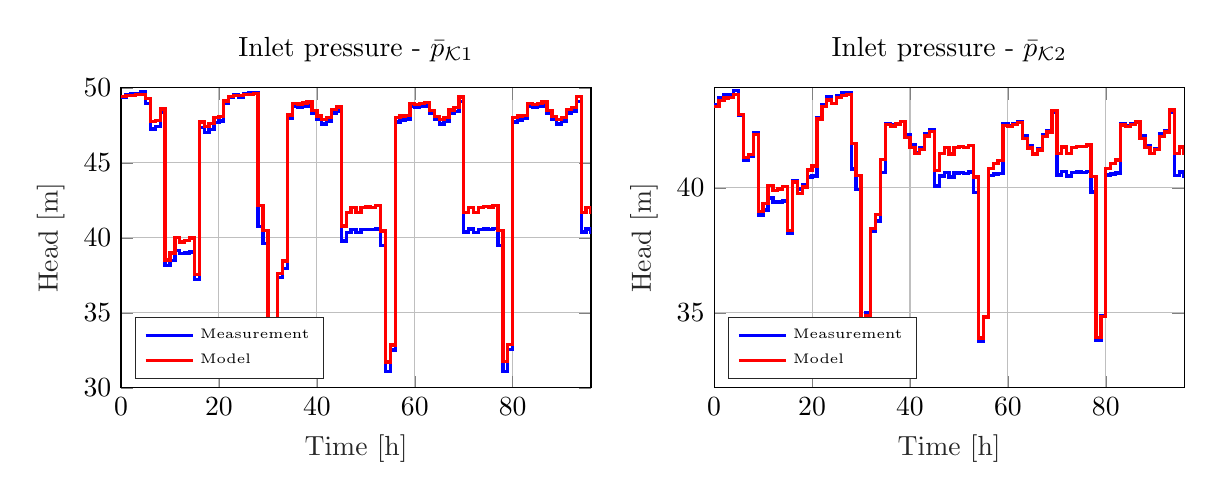
\begin{tikzpicture}

\begin{axis}[%
width=2.35in,
height=1.5in,
at={(0.905in,0.43in)},
scale only axis,
xmin=0,
xmax=96,
xlabel style={font=\color{white!15!black}},
xlabel={Time [h]},
ymin=30,
ymax=50,
grid,
ylabel style={font=\color{white!15!black}},
ylabel={Head  [m]},
axis background/.style={fill=white},
title style={},
title={Inlet pressure - $\bar{p}_{\mathcal{K}1}$},
legend style={at={(0.03,0.03)}, anchor=south west, legend cell align=left, align=left, draw=white!15!black}
]
\addplot[const plot, color=blue, line width=1.2pt] table[row sep=crcr] {%
0	49.36\\
1	49.58\\
2	49.64\\
3	49.64\\
4	49.75\\
5	48.97\\
6	47.25\\
7	47.44\\
8	48.35\\
9	38.18\\
10	38.5\\
11	39.18\\
12	38.95\\
13	38.99\\
14	39.06\\
15	37.23\\
16	47.38\\
17	47.02\\
18	47.23\\
19	47.69\\
20	47.79\\
21	48.97\\
22	49.36\\
23	49.58\\
24	49.39\\
25	49.61\\
26	49.67\\
27	49.67\\
28	40.74\\
29	39.61\\
30	31.21\\
31	32.65\\
32	37.34\\
33	37.94\\
34	47.94\\
35	48.77\\
36	48.71\\
37	48.75\\
38	48.8\\
39	48.3\\
40	47.92\\
41	47.6\\
42	47.8\\
43	48.32\\
44	48.45\\
45	39.79\\
46	40.37\\
47	40.57\\
48	40.34\\
49	40.54\\
50	40.57\\
51	40.54\\
52	40.6\\
53	39.48\\
54	31.08\\
55	32.52\\
56	47.72\\
57	47.85\\
58	47.93\\
59	48.76\\
60	48.7\\
61	48.74\\
62	48.79\\
63	48.29\\
64	47.91\\
65	47.59\\
66	47.79\\
67	48.32\\
68	48.44\\
69	49.07\\
70	40.4\\
71	40.6\\
72	40.37\\
73	40.57\\
74	40.6\\
75	40.57\\
76	40.63\\
77	39.51\\
78	31.11\\
79	32.55\\
80	47.73\\
81	47.86\\
82	47.94\\
83	48.76\\
84	48.7\\
85	48.74\\
86	48.8\\
87	48.3\\
88	47.91\\
89	47.6\\
90	47.79\\
91	48.32\\
92	48.45\\
93	49.07\\
94	40.39\\
95	40.59\\
96	40.36\\
97	40.56\\
98	40.59\\
99	40.57\\
100	40.62\\
101	39.5\\
102	31.1\\
103	32.54\\
104	47.73\\
105	47.86\\
106	47.93\\
107	48.76\\
108	48.7\\
109	48.74\\
110	48.8\\
111	48.29\\
112	47.91\\
113	47.6\\
114	47.79\\
115	48.32\\
116	48.45\\
117	49.07\\
118	40.39\\
119	40.6\\
120	40.36\\
121	40.57\\
122	40.59\\
123	40.57\\
124	40.63\\
125	39.5\\
126	31.1\\
127	32.54\\
128	47.73\\
129	47.86\\
130	47.93\\
131	48.76\\
132	48.7\\
133	48.74\\
134	48.8\\
135	48.29\\
136	47.91\\
137	47.6\\
138	47.79\\
139	48.32\\
140	48.45\\
141	49.07\\
142	40.39\\
143	40.6\\
144	40.36\\
145	40.56\\
146	40.59\\
147	40.57\\
};
\addlegendentry{\tiny Measurement}

\addplot[const plot, color=red, line width=1.2pt] table[row sep=crcr] {%
0	49.407826609926\\
1	49.4752727734975\\
2	49.5002305709133\\
3	49.538153028058\\
4	49.5393266309179\\
5	49.2881540046487\\
6	47.7387112248968\\
7	47.834886272134\\
8	48.6000715782224\\
9	38.5241506873204\\
10	39.0016259346869\\
11	40.0143665682743\\
12	39.7320032884541\\
13	39.8310077454704\\
14	39.9817196522799\\
15	37.5634416507967\\
16	47.7249405342216\\
17	47.4165459163465\\
18	47.602623312586\\
19	48.0208352075825\\
20	48.0936368986064\\
21	49.1252669065493\\
22	49.4139405780143\\
23	49.4819565338709\\
24	49.4890577030841\\
25	49.548410050243\\
26	49.5736581196208\\
27	49.6130406234808\\
28	42.1719362561795\\
29	40.506454401088\\
30	31.7542256801364\\
31	32.8941885640724\\
32	37.6419316114587\\
33	38.4599490202015\\
34	48.1813392155256\\
35	48.9664273993692\\
36	48.9244896970963\\
37	48.9890365002563\\
38	49.0675620743896\\
39	48.4949789896502\\
40	48.1171134727472\\
41	47.8934132319992\\
42	48.0353344401466\\
43	48.5550893552314\\
44	48.7229640821414\\
45	40.7872753923101\\
46	41.6966355832743\\
47	42.020030036948\\
48	41.6889461102772\\
49	42.0126288424584\\
50	42.0671824313218\\
51	42.0440822277871\\
52	42.1384529202662\\
53	40.4687312628601\\
54	31.7324003177415\\
55	32.8681478672251\\
56	48.0400572753494\\
57	48.133075528386\\
58	48.1737785300375\\
59	48.9430148532429\\
60	48.8944027011548\\
61	48.9596354724475\\
62	49.0445726310546\\
63	48.4698620410831\\
64	48.096046109435\\
65	47.872333452587\\
66	48.010930459706\\
67	48.5301597702735\\
68	48.6979611600173\\
69	49.4006015124081\\
70	41.7043121855626\\
71	42.0274182804178\\
72	41.6966355832743\\
73	42.020030036948\\
74	42.0745088055741\\
75	42.053895104588\\
76	42.1456517181628\\
77	40.4795370777088\\
78	31.7370953758699\\
79	32.8756107505396\\
80	48.0441933805401\\
81	48.1354342691993\\
82	48.1763025739849\\
83	48.9516534449101\\
84	48.9072284383221\\
85	48.9723702963734\\
86	49.0530394854694\\
87	48.4782498176924\\
88	48.1075545154378\\
89	47.8793746720474\\
90	48.0219950809957\\
91	48.540641297742\\
92	48.7084231390984\\
93	49.4125774891912\\
94	41.7017547494411\\
95	42.0249569728061\\
96	41.6940738547272\\
97	42.0175644101746\\
98	42.0720681199542\\
99	42.0514440417808\\
100	42.1456517181628\\
101	40.4768377031264\\
102	31.7355314566853\\
103	32.8737467274402\\
104	48.0421272281788\\
105	48.136492610014\\
106	48.1763025739849\\
107	48.9496694789075\\
108	48.9030588630636\\
109	48.9677741379819\\
110	49.0511123026124\\
111	48.4782498176924\\
112	48.1038499492038\\
113	47.8793746720474\\
114	48.0168016543838\\
115	48.5384462371149\\
116	48.7062900724408\\
117	49.4084872968006\\
118	41.7043121855626\\
119	42.0274182804178\\
120	41.6940738547272\\
121	42.0175644101746\\
122	42.0720681199542\\
123	42.0514440417808\\
124	42.1456517181628\\
125	40.4768377031264\\
126	31.7370953758699\\
127	32.8737467274402\\
128	48.0454728307479\\
129	48.136492610014\\
130	48.1763025739849\\
131	48.9516534449101\\
132	48.9030588630636\\
133	48.9719374105997\\
134	49.0511123026124\\
135	48.4782498176924\\
136	48.1038499492038\\
137	47.8793746720474\\
138	48.0191035972588\\
139	48.5384462371149\\
140	48.7062900724408\\
141	49.4084872968006\\
142	41.7017547494411\\
143	42.0274182804178\\
144	41.6940738547272\\
145	42.0175644101746\\
146	42.0720681199542\\
147	42.0514440417808\\
};
\addlegendentry{\tiny Model}

\end{axis}

\begin{axis}[%
xshift=-0.25cm,
width=2.35in,
height=1.5in,
at={(3.969in,0.43in)},
scale only axis,
xmin=0,
xmax=96,
grid,
xlabel style={font=\color{white!15!black}},
xlabel={Time [h]},
ymin=32,
ymax=44,
ylabel style={font=\color{white!15!black}},
ylabel={Head  [m]},
axis background/.style={fill=white},
title style={},
title={Inlet pressure - $\bar{p}_{\mathcal{K}2}$},
legend style={at={(0.03,0.03)}, anchor=south west, legend cell align=left, align=left, draw=white!15!black}
]
\addplot[const plot, color=blue, line width=1.2pt] table[row sep=crcr] {%
0	43.31\\
1	43.62\\
2	43.72\\
3	43.73\\
4	43.9\\
5	42.89\\
6	41.11\\
7	41.28\\
8	42.21\\
9	38.91\\
10	39.12\\
11	39.6\\
12	39.43\\
13	39.44\\
14	39.48\\
15	38.17\\
16	40.3\\
17	39.95\\
18	40.14\\
19	40.44\\
20	40.48\\
21	42.79\\
22	43.31\\
23	43.63\\
24	43.38\\
25	43.69\\
26	43.79\\
27	43.81\\
28	40.76\\
29	39.94\\
30	34.01\\
31	34.99\\
32	38.26\\
33	38.67\\
34	40.61\\
35	42.57\\
36	42.51\\
37	42.57\\
38	42.65\\
39	42.11\\
40	41.71\\
41	41.4\\
42	41.6\\
43	42.17\\
44	42.31\\
45	40.07\\
46	40.48\\
47	40.62\\
48	40.44\\
49	40.59\\
50	40.61\\
51	40.58\\
52	40.63\\
53	39.81\\
54	33.88\\
55	34.85\\
56	40.5\\
57	40.55\\
58	40.58\\
59	42.55\\
60	42.49\\
61	42.55\\
62	42.63\\
63	42.09\\
64	41.69\\
65	41.37\\
66	41.57\\
67	42.14\\
68	42.29\\
69	43.03\\
70	40.51\\
71	40.65\\
72	40.48\\
73	40.62\\
74	40.64\\
75	40.62\\
76	40.66\\
77	39.84\\
78	33.91\\
79	34.89\\
80	40.51\\
81	40.56\\
82	40.59\\
83	42.55\\
84	42.5\\
85	42.56\\
86	42.64\\
87	42.1\\
88	41.7\\
89	41.38\\
90	41.58\\
91	42.15\\
92	42.3\\
93	43.04\\
94	40.5\\
95	40.64\\
96	40.47\\
97	40.61\\
98	40.63\\
99	40.61\\
100	40.65\\
101	39.83\\
102	33.9\\
103	34.88\\
104	40.51\\
105	40.56\\
106	40.59\\
107	42.55\\
108	42.49\\
109	42.56\\
110	42.64\\
111	42.09\\
112	41.7\\
113	41.38\\
114	41.58\\
115	42.15\\
116	42.3\\
117	43.03\\
118	40.5\\
119	40.65\\
120	40.47\\
121	40.61\\
122	40.63\\
123	40.61\\
124	40.65\\
125	39.83\\
126	33.9\\
127	34.88\\
128	40.51\\
129	40.56\\
130	40.59\\
131	42.55\\
132	42.49\\
133	42.56\\
134	42.64\\
135	42.09\\
136	41.7\\
137	41.38\\
138	41.58\\
139	42.15\\
140	42.3\\
141	43.03\\
142	40.5\\
143	40.65\\
144	40.47\\
145	40.61\\
146	40.63\\
147	40.61\\
};
\addlegendentry{\tiny Measurement}

\addplot[const plot, color=red, line width=1.2pt] table[row sep=crcr] {%
0	43.2562476156758\\
1	43.5067171389358\\
2	43.5907578489515\\
3	43.6266462235226\\
4	43.7420185063715\\
5	42.9400970843203\\
6	41.2169651698565\\
7	41.32809131811\\
8	42.1295655117065\\
9	39.0560765750065\\
10	39.3857951432196\\
11	40.1067873335315\\
12	39.8905017535109\\
13	39.9507447729979\\
14	40.0486031467443\\
15	38.2946648361254\\
16	40.2360422251685\\
17	39.7722905159228\\
18	40.0327854424037\\
19	40.7182614307721\\
20	40.8778440485792\\
21	42.7552664453962\\
22	43.2650752039372\\
23	43.5160871329708\\
24	43.3622382186491\\
25	43.6076705705172\\
26	43.6934082607975\\
27	43.7319153025323\\
28	41.7662796742224\\
29	40.4996234450301\\
30	34.0472237341774\\
31	34.8999634656097\\
32	38.3656866100663\\
33	38.9405692080318\\
34	41.1254335719792\\
35	42.5330104693806\\
36	42.4804400279611\\
37	42.5581051250796\\
38	42.6552834610548\\
39	42.005885110475\\
40	41.620385777336\\
41	41.3866029398933\\
42	41.5402164404278\\
43	42.077446618395\\
44	42.2597139762973\\
45	40.7025779071857\\
46	41.3733160616652\\
47	41.6210947850192\\
48	41.35906844914\\
49	41.6070264236885\\
50	41.6489213669406\\
51	41.6245838935181\\
52	41.7013045076067\\
53	40.4320065182672\\
54	33.9903200023213\\
55	34.8402261547627\\
56	40.766337429095\\
57	40.9809171437492\\
58	41.1056198608744\\
59	42.5048654855407\\
60	42.4432011957792\\
61	42.5229894132158\\
62	42.6274378249097\\
63	41.975476911779\\
64	41.5929646794838\\
65	41.3596946357845\\
66	41.5094326729388\\
67	42.048901812441\\
68	42.2309707708959\\
69	43.0959534257937\\
70	41.3875522444622\\
71	41.63515165198\\
72	41.3733160616652\\
73	41.6210947850192\\
74	41.6629434445865\\
75	41.6433103107386\\
76	41.7152488785733\\
77	40.4513504307114\\
78	34.0025306497105\\
79	34.8573150513181\\
80	40.7789902826358\\
81	40.9874246440075\\
82	41.1122271623611\\
83	42.5153744871205\\
84	42.4594816729474\\
85	42.5392160552442\\
86	42.6378264035759\\
87	41.9856236761905\\
88	41.608035365202\\
89	41.368674184251\\
90	41.524157279132\\
91	42.0603558866289\\
92	42.240763352761\\
93	43.1117361709041\\
94	41.3828081209613\\
95	41.6304673075997\\
96	41.3685681268407\\
97	41.6164066077748\\
98	41.6582706962059\\
99	41.6386306210723\\
100	41.7152488785733\\
101	40.4465163092241\\
102	33.9984614619816\\
103	34.8530444068345\\
104	40.772665204556\\
105	40.9862153062005\\
106	41.1122271623611\\
107	42.5140197274845\\
108	42.453698258538\\
109	42.5314623117378\\
110	42.6365124451204\\
111	41.9856236761905\\
112	41.6025734191644\\
113	41.368674184251\\
114	41.5161580267173\\
115	42.0589780905954\\
116	42.239400362466\\
117	43.1060054200663\\
118	41.3875522444622\\
119	41.63515165198\\
120	41.3685681268407\\
121	41.6164066077748\\
122	41.6582706962059\\
123	41.6386306210723\\
124	41.7152488785733\\
125	40.4465163092241\\
126	34.0025306497105\\
127	34.8530444068345\\
128	40.7779137417133\\
129	40.9862153062005\\
130	41.1122271623611\\
131	42.5153744871205\\
132	42.453698258538\\
133	42.5372412651019\\
134	42.6365124451204\\
135	41.9856236761905\\
136	41.6025734191644\\
137	41.368674184251\\
138	41.5175118822089\\
139	42.0589780905954\\
140	42.239400362466\\
141	43.1060054200663\\
142	41.3828081209613\\
143	41.63515165198\\
144	41.3685681268407\\
145	41.6164066077748\\
146	41.6582706962059\\
147	41.6386306210723\\
};
\addlegendentry{\tiny Model}

\end{axis}
\end{tikzpicture}% 
 \vspace{-2.5mm}
 \caption{Validation 1.}
 \label{fig:pk_v1_ident}
 \end{figure}

 \vspace{-4mm}

 In \figref{fig:pk_v1_ident}, the largest difference between the measurement data and the model is at times when both pumping stations shut down. Although at these times the inlet flow is zero, the model reacts well for the changes of the total consumption and the pressure in the WT.

  \vspace{-2mm}

   %pk1 - pk2 v1
 \begin{figure}[H]
 \centering
 %\hspace{-10mm}
 %
\includegraphics[width=0.35\textwidth]{report/pictures/missingfigure}
 % This file was created by matlab2tikz.
%
%The latest updates can be retrieved from
%  http://www.mathworks.com/matlabcentral/fileexchange/22022-matlab2tikz-matlab2tikz
%where you can also make suggestions and rate matlab2tikz.
%
\definecolor{mycolor1}{rgb}{0.00000,0.44700,0.74100}%
\definecolor{mycolor2}{rgb}{0.85000,0.32500,0.09800}%
%
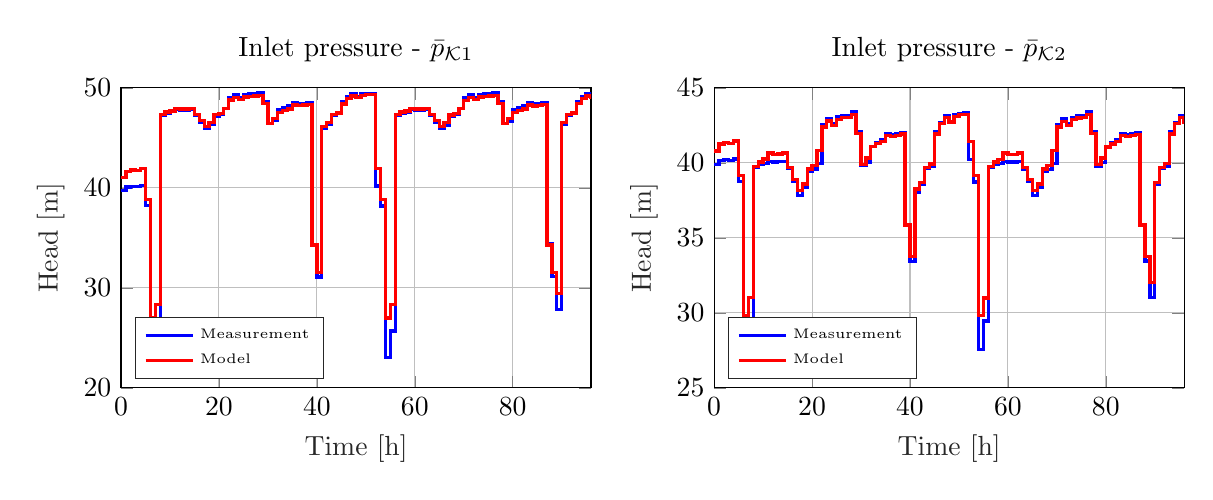
\begin{tikzpicture}

\begin{axis}[%
width=2.35in,
height=1.5in,
at={(0.905in,0.43in)},
scale only axis,
xmin=0,
xmax=96,
xlabel style={font=\color{white!15!black}},
xlabel={Time [h]},
ymin=20,
ymax=50,
grid,
ylabel style={font=\color{white!15!black}},
ylabel={Head  [m]},
axis background/.style={fill=white},
title style={},
title={Inlet pressure - $\bar{p}_{\mathcal{K}1}$},
legend style={at={(0.03,0.03)}, anchor=south west, legend cell align=left, align=left, draw=white!15!black}
]
\addplot[const plot, color=blue, line width=1.2pt] table[row sep=crcr] {%
0	39.73\\
1	40.1\\
2	40.15\\
3	40.11\\
4	40.22\\
5	38.22\\
6	23.08\\
7	25.72\\
8	47.28\\
9	47.49\\
10	47.61\\
11	47.84\\
12	47.78\\
13	47.8\\
14	47.83\\
15	47.23\\
16	46.59\\
17	45.93\\
18	46.31\\
19	47.17\\
20	47.33\\
21	47.93\\
22	49.05\\
23	49.32\\
24	49.07\\
25	49.35\\
26	49.42\\
27	49.42\\
28	49.55\\
29	48.6\\
30	46.45\\
31	46.71\\
32	47.81\\
33	48.04\\
34	48.18\\
35	48.49\\
36	48.42\\
37	48.46\\
38	48.52\\
39	34.37\\
40	31.09\\
41	46\\
42	46.38\\
43	47.24\\
44	47.41\\
45	48.64\\
46	49.1\\
47	49.38\\
48	49.13\\
49	49.4\\
50	49.47\\
51	49.47\\
52	40.19\\
53	38.19\\
54	23.05\\
55	25.69\\
56	47.28\\
57	47.49\\
58	47.6\\
59	47.83\\
60	47.77\\
61	47.79\\
62	47.83\\
63	47.23\\
64	46.58\\
65	45.93\\
66	46.3\\
67	47.16\\
68	47.33\\
69	47.93\\
70	49.04\\
71	49.32\\
72	49.07\\
73	49.34\\
74	49.42\\
75	49.41\\
76	49.55\\
77	48.6\\
78	46.45\\
79	46.7\\
80	47.8\\
81	48.03\\
82	48.18\\
83	48.48\\
84	48.41\\
85	48.46\\
86	48.51\\
87	34.4\\
88	31.11\\
89	27.83\\
90	46.38\\
91	47.24\\
92	47.41\\
93	48.65\\
94	49.11\\
95	49.38\\
96	49.13\\
97	49.4\\
98	49.48\\
99	49.47\\
100	40.19\\
101	38.19\\
102	23.05\\
103	25.69\\
104	47.28\\
105	47.49\\
106	47.6\\
107	47.83\\
108	47.77\\
109	47.79\\
110	47.83\\
111	47.23\\
112	46.58\\
113	45.92\\
114	46.3\\
115	47.16\\
116	47.32\\
117	47.92\\
118	49.04\\
119	49.32\\
120	49.07\\
121	49.34\\
122	49.42\\
123	49.41\\
124	49.55\\
125	48.6\\
126	46.45\\
127	46.7\\
128	47.8\\
129	48.03\\
130	48.18\\
131	48.48\\
132	48.41\\
133	48.46\\
134	48.51\\
135	34.4\\
136	31.11\\
137	27.83\\
138	46.38\\
139	47.24\\
140	47.41\\
141	48.65\\
142	49.11\\
143	49.38\\
144	49.13\\
145	49.4\\
146	49.48\\
147	49.47\\
};
\addlegendentry{\tiny Measurement}

\addplot[const plot, color=red, line width=1.2pt] table[row sep=crcr] {%
0	41.0291872224712\\
1	41.6648509305914\\
2	41.7778226171809\\
3	41.7356088694338\\
4	41.9303664739708\\
5	38.8222805362074\\
6	26.9960296847917\\
7	28.3197940460292\\
8	47.3548724532373\\
9	47.5744143197647\\
10	47.6986920757271\\
11	47.933688094449\\
12	47.8791046240103\\
13	47.8990451139347\\
14	47.9291366985189\\
15	47.3280698571769\\
16	46.7481922263548\\
17	46.133687961783\\
18	46.524915203528\\
19	47.3063777534193\\
20	47.4680277600409\\
21	47.9695910597047\\
22	48.7845477782499\\
23	49.0186491881492\\
24	48.8702851350243\\
25	49.0969893467872\\
26	49.1606333462978\\
27	49.1945896219237\\
28	49.254195339467\\
29	48.440618696435\\
30	46.4581008063898\\
31	46.9203794351619\\
32	47.5450581982503\\
33	47.7435243962032\\
34	47.9009777379091\\
35	48.2891232292179\\
36	48.21030564654\\
37	48.2782623951455\\
38	48.3669754567863\\
39	34.285504859126\\
40	31.5480196601649\\
41	46.1222605854113\\
42	46.5241242479027\\
43	47.329725808184\\
44	47.4986161586634\\
45	48.403877984095\\
46	48.9633364372308\\
47	49.1818461364568\\
48	49.0447057753511\\
49	49.2575213529045\\
50	49.3149585759289\\
51	49.3488749596997\\
52	41.9253311556918\\
53	38.8140761438897\\
54	26.9961096933227\\
55	28.3182838302489\\
56	47.354027591064\\
57	47.5730658304846\\
58	47.6970416155644\\
59	47.9291366985189\\
60	47.8735721019748\\
61	47.8946800203324\\
62	47.9268553538656\\
63	47.324324891826\\
64	46.7485108842582\\
65	46.1334191818822\\
66	46.5236328238201\\
67	47.3025463019357\\
68	47.4667416197553\\
69	47.9675536464269\\
70	48.7714725609738\\
71	49.0049396696284\\
72	48.8555077501858\\
73	49.0875729716479\\
74	49.1489337914536\\
75	49.1828960142227\\
76	49.2430975084357\\
77	48.4252125039367\\
78	46.4560258826819\\
79	46.9152543915797\\
80	47.5348713769164\\
81	47.729045818393\\
82	47.8886155989533\\
83	48.2780384615744\\
84	48.1975716076942\\
85	48.26552490802\\
86	48.3583278059229\\
87	34.2898992188893\\
88	31.5511648686405\\
89	29.4713680397618\\
90	46.5233960151711\\
91	47.330548221374\\
92	47.4998310485311\\
93	48.4107976349701\\
94	48.9700693407683\\
95	49.1881833951118\\
96	49.0531009857387\\
97	49.2629384856557\\
98	49.3223055415088\\
99	49.3562133051815\\
100	41.9228113786962\\
101	38.8140761438897\\
102	26.9961483054671\\
103	28.3182838302489\\
104	47.3511084177016\\
105	47.5730658304846\\
106	47.6970416155644\\
107	47.9291366985189\\
108	47.8735721019748\\
109	47.8946800203324\\
110	47.9268553538656\\
111	47.324324891826\\
112	46.7463013015267\\
113	46.1334191818822\\
114	46.5236328238201\\
115	47.3025463019357\\
116	47.4667416197553\\
117	47.9639817997383\\
118	48.7695673232379\\
119	49.0049396696284\\
120	48.8555077501858\\
121	49.0834873112628\\
122	49.1489337914536\\
123	49.1828960142227\\
124	49.2430975084357\\
125	48.4249845430264\\
126	46.4580576784382\\
127	46.9152543915797\\
128	47.5313177315955\\
129	47.729045818393\\
130	47.8861858713391\\
131	48.2780172937153\\
132	48.1975716076942\\
133	48.2632154274819\\
134	48.3542173796042\\
135	34.2898992188893\\
136	31.5511648686405\\
137	29.472297795143\\
138	46.5233960151711\\
139	47.330548221374\\
140	47.4998310485311\\
141	48.4107976349701\\
142	48.9718666250928\\
143	49.1922421381702\\
144	49.0531009857387\\
145	49.2678016300303\\
146	49.3223055415088\\
147	49.3562133051815\\
};
\addlegendentry{\tiny Model}

\end{axis}

\begin{axis}[%
width=2.35in,
height=1.5in,
xshift=-0.25cm,
at={(3.969in,0.43in)},
scale only axis,
xmin=0,
xmax=96,
grid,
xlabel style={font=\color{white!15!black}},
xlabel={Time [h]},
ymin=25,
ymax=45,
ylabel style={font=\color{white!15!black}},
ylabel={Head  [m]},
axis background/.style={fill=white},
title style={},
title={Inlet pressure - $\bar{p}_{\mathcal{K}2}$},
legend style={at={(0.03,0.03)}, anchor=south west, legend cell align=left, align=left, draw=white!15!black}
]
\addplot[const plot, color=blue, line width=1.2pt] table[row sep=crcr] {%
0	39.9\\
1	40.18\\
2	40.22\\
3	40.18\\
4	40.26\\
5	38.75\\
6	27.59\\
7	29.48\\
8	39.71\\
9	39.9\\
10	39.98\\
11	40.1\\
12	40.06\\
13	40.07\\
14	40.09\\
15	39.61\\
16	38.8\\
17	37.84\\
18	38.37\\
19	39.44\\
20	39.59\\
21	39.97\\
22	42.55\\
23	42.98\\
24	42.62\\
25	43.05\\
26	43.18\\
27	43.18\\
28	43.4\\
29	42.07\\
30	39.81\\
31	40.05\\
32	41.1\\
33	41.37\\
34	41.56\\
35	41.94\\
36	41.87\\
37	41.93\\
38	42.01\\
39	35.88\\
40	33.44\\
41	38.02\\
42	38.55\\
43	39.63\\
44	39.78\\
45	42.05\\
46	42.7\\
47	43.12\\
48	42.77\\
49	43.19\\
50	43.31\\
51	43.32\\
52	40.24\\
53	38.72\\
54	27.56\\
55	29.46\\
56	39.69\\
57	39.89\\
58	39.96\\
59	40.09\\
60	40.05\\
61	40.06\\
62	40.07\\
63	39.6\\
64	38.79\\
65	37.83\\
66	38.36\\
67	39.43\\
68	39.58\\
69	39.96\\
70	42.54\\
71	42.97\\
72	42.62\\
73	43.04\\
74	43.17\\
75	43.17\\
76	43.39\\
77	42.06\\
78	39.8\\
79	40.04\\
80	41.09\\
81	41.36\\
82	41.55\\
83	41.93\\
84	41.86\\
85	41.92\\
86	42\\
87	35.9\\
88	33.46\\
89	31.03\\
90	38.56\\
91	39.64\\
92	39.79\\
93	42.06\\
94	42.71\\
95	43.13\\
96	42.78\\
97	43.19\\
98	43.32\\
99	43.32\\
100	40.23\\
101	38.71\\
102	27.56\\
103	29.45\\
104	39.69\\
105	39.89\\
106	39.96\\
107	40.09\\
108	40.05\\
109	40.06\\
110	40.07\\
111	39.6\\
112	38.78\\
113	37.83\\
114	38.35\\
115	39.43\\
116	39.58\\
117	39.95\\
118	42.54\\
119	42.97\\
120	42.61\\
121	43.04\\
122	43.17\\
123	43.17\\
124	43.39\\
125	42.06\\
126	39.79\\
127	40.04\\
128	41.09\\
129	41.36\\
130	41.55\\
131	41.93\\
132	41.86\\
133	41.92\\
134	42\\
135	35.9\\
136	33.46\\
137	31.03\\
138	38.56\\
139	39.64\\
140	39.79\\
141	42.06\\
142	42.71\\
143	43.13\\
144	42.78\\
145	43.19\\
146	43.32\\
147	43.32\\
};
\addlegendentry{\tiny Measurement}

\addplot[const plot, color=red, line width=1.2pt] table[row sep=crcr] {%
0	40.787128700406\\
1	41.2570074568191\\
2	41.3417021544305\\
3	41.3033281480082\\
4	41.451519467749\\
5	39.1554509035734\\
6	29.8191037973752\\
7	31.0086559797237\\
8	39.7593312509542\\
9	40.066907796094\\
10	40.2512684077171\\
11	40.6678909266222\\
12	40.5522441258968\\
13	40.5930448326794\\
14	40.6549589571521\\
15	39.6907992421198\\
16	38.9107856014093\\
17	38.1725199439454\\
18	38.5934686278776\\
19	39.5929084054844\\
20	39.8198406810546\\
21	40.8226793140286\\
22	42.4020369902975\\
23	42.7944490131123\\
24	42.5058641706844\\
25	42.8939275328576\\
26	43.0165308923596\\
27	43.0464139194099\\
28	43.2222917330325\\
29	41.9786335438016\\
30	39.8829433447864\\
31	40.3316998299902\\
32	41.0756270365695\\
33	41.2780481573897\\
34	41.4369071827189\\
35	41.8267970131656\\
36	41.7522522112771\\
37	41.8258890610217\\
38	41.9199463498011\\
39	35.8480981436472\\
40	33.7370741079152\\
41	38.2521702644172\\
42	38.6810639858498\\
43	39.7018151967257\\
44	39.9337113343167\\
45	41.9206214187225\\
46	42.6193761962468\\
47	43.002606319134\\
48	42.7200655757163\\
49	43.1001763013893\\
50	43.2172509212131\\
51	43.2469494687578\\
52	41.442050528313\\
53	39.1408624276459\\
54	29.8130582243956\\
55	30.998504202922\\
56	39.7538117963779\\
57	40.0610446110157\\
58	40.2452041464504\\
59	40.6549589571521\\
60	40.540574998224\\
61	40.5802289476738\\
62	40.6484889556866\\
63	39.6803236605887\\
64	38.9061006590988\\
65	38.1645009156898\\
66	38.5847184710748\\
67	39.582370385981\\
68	39.8140169199104\\
69	40.8145036433266\\
70	42.3854170627495\\
71	42.7771858688424\\
72	42.4880049970651\\
73	42.8825673106501\\
74	43.0007682577757\\
75	43.0306637603329\\
76	43.2069220649113\\
77	41.9606833524876\\
78	39.8776767528089\\
79	40.3246061044158\\
80	41.0646487851362\\
81	41.2610833972401\\
82	41.4211637840973\\
83	41.81483247685\\
84	41.7361741703017\\
85	41.8097965024625\\
86	41.909563675917\\
87	35.8570961434983\\
88	33.7452476866249\\
89	32.0123269861868\\
90	38.6854434327548\\
91	39.7073192906508\\
92	39.9394848961065\\
93	41.9299475436721\\
94	42.6286212208108\\
95	43.0115950686304\\
96	42.7305221920427\\
97	43.106963736353\\
98	43.2270673251283\\
99	43.2567534491557\\
100	41.4373141696299\\
101	39.1408624276459\\
102	29.8100341111194\\
103	30.998504202922\\
104	39.748844092779\\
105	40.0610446110157\\
106	40.2452041464504\\
107	40.6549589571521\\
108	40.540574998224\\
109	40.5802289476738\\
110	40.6484889556866\\
111	39.6803236605887\\
112	38.9016021615105\\
113	38.1645009156898\\
114	38.5847184710748\\
115	39.582370385981\\
116	39.8140169199104\\
117	40.8090874211475\\
118	42.3840323693096\\
119	42.7771858688424\\
120	42.4880049970651\\
121	42.8768137126139\\
122	43.0007682577757\\
123	43.0306637603329\\
124	43.2069220649113\\
125	41.9588335734523\\
126	39.8776111164751\\
127	40.3246061044158\\
128	41.0592779455444\\
129	41.2610833972401\\
130	41.4196543416304\\
131	41.8131073756464\\
132	41.7361741703017\\
133	41.8083161130909\\
134	41.9021079252652\\
135	35.8570961434983\\
136	33.7452476866249\\
137	32.015991779775\\
138	38.6854434327548\\
139	39.7073192906508\\
140	39.9394848961065\\
141	41.9299475436721\\
142	42.6299280603166\\
143	43.0173277101085\\
144	42.7305221920427\\
145	43.1148148575598\\
146	43.2270673251283\\
147	43.2567534491557\\
};
\addlegendentry{\tiny Model}

\end{axis}
\end{tikzpicture}% 
 \vspace{-2.5mm}
 \caption{Validation 2.}
 \label{fig:pk_v2_ident}
 \end{figure}

 \vspace{-4mm}

In \figref{fig:pk_v2_ident}, the model shows good results in case if the pumps shut down and turn on for different WT levels and inlet pressures. Similarly to Validation 1, the biggest difference between the model and measurement are at times when both pumps are completely shut down. 

 \subsection{State model}
 \label{state_model}

For the WT pressure $\hat{p}$, the identification has been carried out with five RBF neurons on the difference of the current and the next pressure head. \figref{fig:MSE_state}shows the mean squared errors in terms of RBF neurons on the identified network model.

\vspace{-1mm}

  %MSE state
 \begin{figure}[H]
 \centering
 %\hspace{0mm}
 %
\includegraphics[width=0.35\textwidth]{report/pictures/missingfigure}
 % This file was created by matlab2tikz.
%
%The latest updates can be retrieved from
%  http://www.mathworks.com/matlabcentral/fileexchange/22022-matlab2tikz-matlab2tikz
%where you can also make suggestions and rate matlab2tikz.
%
\definecolor{mycolor1}{rgb}{0.92900,0.69400,0.12500}%
\definecolor{mycolor2}{rgb}{0.49400,0.18400,0.55600}%
%
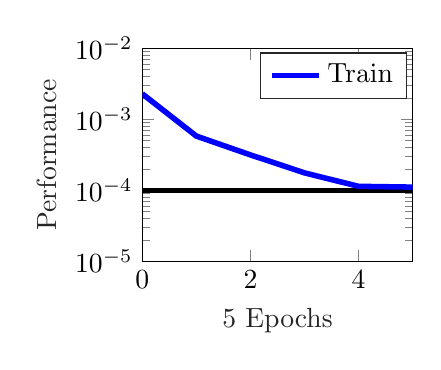
\begin{tikzpicture}

\begin{axis}[%
width=1.3521in,
height=1.066in,
at={(0.758in,0.481in)},
scale only axis,
xmin=0,
xmax=5,
xlabel style={font=\color{white!15!black}},
xlabel={5 Epochs},
ymode=log,
ymin=1e-05,
ymax=0.01,
yminorticks=true,
ylabel style={font=\color{white!15!black}},
ylabel={Performance},
axis background/.style={fill=white},
title style={},
%title={Performance is 0.000110874, Goal is 0.0001},
legend style={legend cell align=left, align=left, draw=white!15!black}
]
\addplot [color=black, line width=2.0pt, forget plot]
  table[row sep=crcr]{%
0	0.0001\\
1	0.0001\\
2	0.0001\\
3	0.0001\\
4	0.0001\\
5	0.0001\\
};
\addplot [color=blue, line width=2.0pt]
  table[row sep=crcr]{%
0	0.00227799032140248\\
1	0.000579231145498518\\
2	0.000314828855310372\\
3	0.000175750288046433\\
4	0.000113694020777771\\
5	0.000110874217700856\\
};
\addlegendentry{Train}

\addplot [color=mycolor1, forget plot]
  table[row sep=crcr]{%
0	0\\
};
\addplot [color=mycolor2, forget plot]
  table[row sep=crcr]{%
0	0\\
};
\end{axis}
\end{tikzpicture}% 
 \vspace{-3.5mm}
 \caption{The network’s performance according to the mean of squared errors.}
 \label{fig:MSE_state}
 \end{figure}

 \vspace{-3mm}

 \figref{fig:MSE_state} shows, that using more neurons in the model, does not improve the performance significantly. The result of identification is shown in \figref{fig:p_WT_ident}. The two validation results are shown in \figref{fig:p_WT_ident_v1} and \figref{fig:p_WT_ident_v2}, respectively. 

   %p_WT (k+1) - p_WT(k)
 \begin{figure}[H]
 \centering
 %\hspace{0mm}
 %
\includegraphics[width=0.35\textwidth]{report/pictures/missingfigure}
 % This file was created by matlab2tikz.
%
%The latest updates can be retrieved from
%  http://www.mathworks.com/matlabcentral/fileexchange/22022-matlab2tikz-matlab2tikz
%where you can also make suggestions and rate matlab2tikz.
%
\definecolor{mycolor1}{rgb}{0.00000,0.44700,0.74100}%
\definecolor{mycolor2}{rgb}{0.85000,0.32500,0.09800}%
%
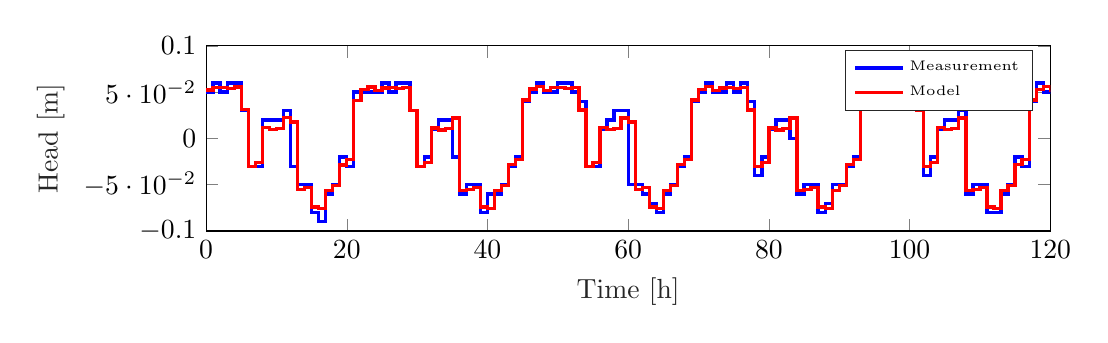
\begin{tikzpicture}

\begin{axis}[%
width=4.221in,
height=0.926in,
at={(0.75in,0.431in)},
scale only axis,
xmin=0,
xmax=120,
xlabel style={font=\color{white!15!black}},
xlabel={Time [h]},
ymin=-0.1,
ymax=0.1,
ylabel style={font=\color{white!15!black}},
ylabel={Head  [m]},
axis background/.style={fill=white},
title style={},
%title={Identification of $\hat{p}^{(k+1)} - \hat{p}^{(k)}$},
legend style={legend cell align=left, align=left, draw=white!15!black}
]
\addplot[const plot, color=blue, line width=1.2pt] table[row sep=crcr] {%
0	0.0500000000000007\\
1	0.0599999999999987\\
2	0.0500000000000007\\
3	0.0599999999999987\\
4	0.0600000000000023\\
5	0.0299999999999976\\
6	-0.0299999999999976\\
7	-0.0300000000000011\\
8	0.0199999999999996\\
9	0.0199999999999996\\
10	0.0199999999999996\\
11	0.0300000000000011\\
12	-0.0300000000000011\\
13	-0.0499999999999972\\
14	-0.0500000000000007\\
15	-0.0800000000000018\\
16	-0.0899999999999999\\
17	-0.0599999999999987\\
18	-0.0500000000000007\\
19	-0.0199999999999996\\
20	-0.0300000000000011\\
21	0.0500000000000007\\
22	0.0500000000000007\\
23	0.0500000000000007\\
24	0.0499999999999972\\
25	0.0600000000000023\\
26	0.0500000000000007\\
27	0.0599999999999987\\
28	0.0599999999999987\\
29	0.0300000000000011\\
30	-0.0300000000000011\\
31	-0.0199999999999996\\
32	0.0100000000000016\\
33	0.0199999999999996\\
34	0.0199999999999996\\
35	-0.0199999999999996\\
36	-0.0599999999999987\\
37	-0.0500000000000007\\
38	-0.0500000000000007\\
39	-0.0800000000000018\\
40	-0.0599999999999987\\
41	-0.0599999999999987\\
42	-0.0500000000000007\\
43	-0.0300000000000011\\
44	-0.0199999999999996\\
45	0.0399999999999991\\
46	0.0500000000000007\\
47	0.0600000000000023\\
48	0.0499999999999972\\
49	0.0500000000000007\\
50	0.0600000000000023\\
51	0.0599999999999987\\
52	0.0500000000000007\\
53	0.0399999999999991\\
54	-0.0300000000000011\\
55	-0.0299999999999976\\
56	0.00999999999999801\\
57	0.0199999999999996\\
58	0.0300000000000011\\
59	0.0300000000000011\\
60	-0.0500000000000007\\
61	-0.0500000000000007\\
62	-0.0599999999999987\\
63	-0.0700000000000003\\
64	-0.0800000000000018\\
65	-0.0599999999999987\\
66	-0.0500000000000007\\
67	-0.0300000000000011\\
68	-0.0199999999999996\\
69	0.0400000000000027\\
70	0.0499999999999972\\
71	0.0600000000000023\\
72	0.0499999999999972\\
73	0.0500000000000007\\
74	0.0600000000000023\\
75	0.0499999999999972\\
76	0.0600000000000023\\
77	0.0399999999999991\\
78	-0.0399999999999991\\
79	-0.0199999999999996\\
80	0.00999999999999801\\
81	0.0199999999999996\\
82	0.0199999999999996\\
83	0\\
84	-0.0599999999999987\\
85	-0.0500000000000007\\
86	-0.0499999999999972\\
87	-0.0800000000000018\\
88	-0.0700000000000003\\
89	-0.0500000000000007\\
90	-0.0499999999999972\\
91	-0.0300000000000011\\
92	-0.0199999999999996\\
93	0.0399999999999991\\
94	0.0500000000000007\\
95	0.0500000000000007\\
96	0.0499999999999972\\
97	0.0600000000000023\\
98	0.0599999999999987\\
99	0.0500000000000007\\
100	0.0599999999999987\\
101	0.0399999999999991\\
102	-0.0399999999999991\\
103	-0.0199999999999996\\
104	0.0100000000000016\\
105	0.0199999999999996\\
106	0.0199999999999996\\
107	0.0300000000000011\\
108	-0.0600000000000023\\
109	-0.0500000000000007\\
110	-0.0499999999999972\\
111	-0.0800000000000018\\
112	-0.0799999999999983\\
113	-0.0600000000000023\\
114	-0.0499999999999972\\
115	-0.0200000000000031\\
116	-0.0299999999999976\\
117	0.0399999999999991\\
118	0.0599999999999987\\
119	0.0500000000000007\\
120	0.0500000000000007\\
121	0.0599999999999987\\
122	0.0500000000000007\\
123	0.0599999999999987\\
124	0.0600000000000023\\
125	0.0299999999999976\\
126	-0.0299999999999976\\
127	-0.0199999999999996\\
128	0.00999999999999801\\
129	0.0199999999999996\\
130	0.0199999999999996\\
131	0\\
132	-0.0499999999999972\\
133	-0.0600000000000023\\
134	-0.0499999999999972\\
135	-0.0700000000000003\\
136	-0.0700000000000003\\
137	-0.0600000000000023\\
138	-0.0499999999999972\\
139	-0.0300000000000011\\
140	-0.0199999999999996\\
141	0.0399999999999991\\
142	0.0500000000000007\\
143	0.0599999999999987\\
144	0.0500000000000007\\
145	0.0500000000000007\\
146	0.0599999999999987\\
147	0.0500000000000007\\
};
\addlegendentry{\tiny Measurement}

\addplot[const plot, color=red, line width=1.2pt] table[row sep=crcr] {%
0	0.0521228227061686\\
1	0.0547770573795134\\
2	0.0549738871275073\\
3	0.0540070332178103\\
4	0.0553581660423539\\
5	0.0309509432175251\\
6	-0.0302541131137425\\
7	-0.0258878149080063\\
8	0.0116835103808151\\
9	0.00944071934988187\\
10	0.0108393467943777\\
11	0.0222620440842331\\
12	0.017753994038684\\
13	-0.0548847444768375\\
14	-0.0529171063665049\\
15	-0.0739347935746965\\
16	-0.075376016348122\\
17	-0.056231715949156\\
18	-0.0509903151309856\\
19	-0.0285570288907828\\
20	-0.0227898729974818\\
21	0.0412596196095969\\
22	0.0530411479359023\\
23	0.0556867071940996\\
24	0.0516831285697461\\
25	0.0544174824153019\\
26	0.0546224036491589\\
27	0.0536576525540963\\
28	0.055021993134575\\
29	0.0305023420618714\\
30	-0.0306695914216996\\
31	-0.0262996522971979\\
32	0.0112312379707287\\
33	0.00904328429132074\\
34	0.0104580081411264\\
35	0.0219038896902016\\
36	-0.0561958592339005\\
37	-0.054885388566092\\
38	-0.0529173406218441\\
39	-0.0739347814363736\\
40	-0.0753754443010152\\
41	-0.056161883307047\\
42	-0.0509213191869045\\
43	-0.0284822230045206\\
44	-0.0227128091088587\\
45	0.0415568554610023\\
46	0.0533317618211848\\
47	0.0559917504950124\\
48	0.0519663524994236\\
49	0.0546880768602094\\
50	0.0548876192171522\\
51	0.0539206880382336\\
52	0.0552751992487784\\
53	0.0308009555503325\\
54	-0.0303552083502845\\
55	-0.025960133451575\\
56	0.011580100345004\\
57	0.00937318604745067\\
58	0.0107453635488297\\
59	0.0221738677095416\\
60	0.0176656824437027\\
61	-0.054884904577296\\
62	-0.0529171833857584\\
63	-0.0739348487680358\\
64	-0.0753759356283361\\
65	-0.056197386588852\\
66	-0.0509903151309856\\
67	-0.0285206521125461\\
68	-0.0227888122974326\\
69	0.0413251192798487\\
70	0.0531068513421642\\
71	0.0557770877829439\\
72	0.0517460048094278\\
73	0.0544777326244898\\
74	0.0546819826563284\\
75	0.0537164614020809\\
76	0.055078693258714\\
77	0.0305905643290179\\
78	-0.0305984619132723\\
79	-0.026227868556545\\
80	0.0113339711794754\\
81	0.00911048667808365\\
82	0.0105223596736294\\
83	0.0219642277572998\\
84	-0.0561956619184653\\
85	-0.0548852910312194\\
86	-0.0529173239390968\\
87	-0.0739348238964695\\
88	-0.0753755923997427\\
89	-0.056161883307047\\
90	-0.0509558574255701\\
91	-0.028483253793275\\
92	-0.0227508388610548\\
93	0.0414884852670658\\
94	0.0532657803134903\\
95	0.0559289087299223\\
96	0.0519663524994236\\
97	0.0546276712915489\\
98	0.0548277821948873\\
99	0.0538614092879333\\
100	0.0552182820271992\\
101	0.0308010226007496\\
102	-0.0304266324209052\\
103	-0.0260581087003671\\
104	0.0115083701013817\\
105	0.00927537805815679\\
106	0.0106806302187197\\
107	0.0221129305878456\\
108	-0.0561952192524557\\
109	-0.0548850490366472\\
110	-0.0529172453209974\\
111	-0.0739348487680358\\
112	-0.07537583806358\\
113	-0.0561968424861917\\
114	-0.0509558574255701\\
115	-0.0285196560373303\\
116	-0.0227888122974326\\
117	0.0413277383550274\\
118	0.0531726671171117\\
119	0.0558383211107313\\
120	0.0518102093792906\\
121	0.0545388978336156\\
122	0.0547410918719858\\
123	0.0537755851554707\\
124	0.0551355122560274\\
125	0.0306514888970745\\
126	-0.0305985384013629\\
127	-0.0261301598518775\\
128	0.0113339711794754\\
129	0.00914063512442724\\
130	0.0105869958831369\\
131	0.0219642277572998\\
132	-0.0561956619184653\\
133	-0.0548851778546835\\
134	-0.0529173239390968\\
135	-0.0739348238964695\\
136	-0.075375723653994\\
137	-0.0561624720089858\\
138	-0.0509558574255701\\
139	-0.028483253793275\\
140	-0.0227508388610548\\
141	0.0414228627586822\\
142	0.0532657803134903\\
143	0.0559289087299223\\
144	0.0519019818943721\\
145	0.0546267548916109\\
146	0.0548277821948873\\
147	0.0538614092879333\\
};
\addlegendentry{\tiny Model}

\end{axis}
\end{tikzpicture}% 
 \vspace{-3.5mm}
 \caption{Identification of $\hat{p}^{(k+1)} - \hat{p}^{(k)}$.}
 \label{fig:p_WT_ident}
 \end{figure}

 \vspace{-4mm}

    %p_WT (k+1) - p_WT(k)
 \begin{figure}[H]
 \centering
 %\hspace{0mm}
 %
\includegraphics[width=0.35\textwidth]{report/pictures/missingfigure}
 % This file was created by matlab2tikz.
%
%The latest updates can be retrieved from
%  http://www.mathworks.com/matlabcentral/fileexchange/22022-matlab2tikz-matlab2tikz
%where you can also make suggestions and rate matlab2tikz.
%
\definecolor{mycolor1}{rgb}{0.00000,0.44700,0.74100}%
\definecolor{mycolor2}{rgb}{0.85000,0.32500,0.09800}%
%
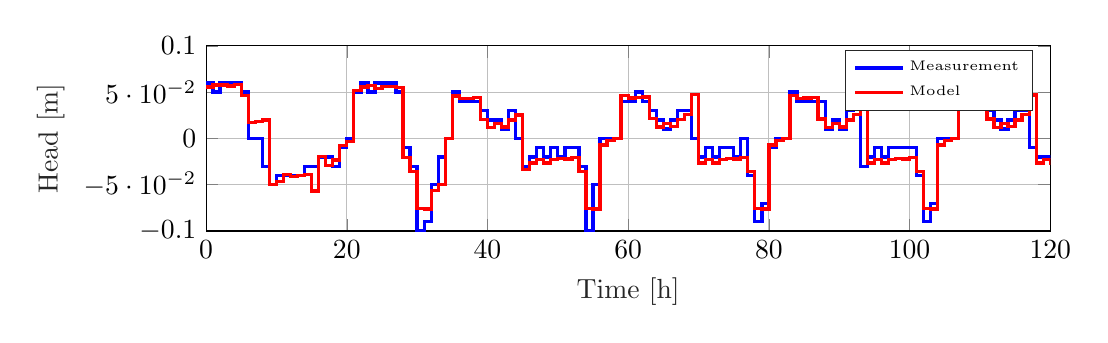
\begin{tikzpicture}

\begin{axis}[%
width=4.221in,
height=0.926in,
at={(0.838in,0.427in)},
scale only axis,
xmin=0,
xmax=120,
xlabel style={font=\color{white!15!black}},
xlabel={Time [h]},
ymin=-0.100000000000001,
ymax=0.1,
grid,
ylabel style={font=\color{white!15!black}},
ylabel={Head  [m]},
axis background/.style={fill=white},
title style={},
%title={'Validation 1' of $\hat{p}^{(k+1)} - \hat{p}^{(k)}$},
legend style={legend cell align=left, align=left, draw=white!15!black}
]
\addplot[const plot, color=blue, line width=1.2pt] table[row sep=crcr] {%
0	0.0599999999999987\\
1	0.0500000000000007\\
2	0.0600000000000023\\
3	0.0599999999999987\\
4	0.0599999999999987\\
5	0.0500000000000007\\
6	0\\
7	0\\
8	-0.0300000000000011\\
9	-0.0499999999999972\\
10	-0.0400000000000027\\
11	-0.0399999999999991\\
12	-0.0399999999999991\\
13	-0.0399999999999991\\
14	-0.0300000000000011\\
15	-0.0300000000000011\\
16	-0.0199999999999996\\
17	-0.0199999999999996\\
18	-0.0300000000000011\\
19	-0.00999999999999801\\
20	0\\
21	0.0500000000000007\\
22	0.0599999999999987\\
23	0.0500000000000007\\
24	0.0599999999999987\\
25	0.0599999999999987\\
26	0.0600000000000023\\
27	0.0500000000000007\\
28	-0.0100000000000016\\
29	-0.0300000000000011\\
30	-0.0999999999999979\\
31	-0.0899999999999999\\
32	-0.0500000000000007\\
33	-0.0199999999999996\\
34	0\\
35	0.0500000000000007\\
36	0.0399999999999991\\
37	0.0399999999999991\\
38	0.0399999999999991\\
39	0.0300000000000011\\
40	0.0199999999999996\\
41	0.0199999999999996\\
42	0.0100000000000016\\
43	0.0299999999999976\\
44	0\\
45	-0.0299999999999976\\
46	-0.0199999999999996\\
47	-0.0100000000000016\\
48	-0.0199999999999996\\
49	-0.0100000000000016\\
50	-0.0199999999999996\\
51	-0.00999999999999801\\
52	-0.0100000000000016\\
53	-0.0299999999999976\\
54	-0.100000000000001\\
55	-0.0500000000000007\\
56	0\\
57	0\\
58	0\\
59	0.0399999999999991\\
60	0.0400000000000027\\
61	0.0499999999999972\\
62	0.0400000000000027\\
63	0.0299999999999976\\
64	0.0199999999999996\\
65	0.0100000000000016\\
66	0.0199999999999996\\
67	0.0300000000000011\\
68	0.0299999999999976\\
69	0\\
70	-0.0199999999999996\\
71	-0.00999999999999801\\
72	-0.0199999999999996\\
73	-0.0100000000000016\\
74	-0.00999999999999801\\
75	-0.0200000000000031\\
76	0\\
77	-0.0399999999999991\\
78	-0.0899999999999999\\
79	-0.0700000000000003\\
80	-0.00999999999999801\\
81	0\\
82	0\\
83	0.0499999999999972\\
84	0.0400000000000027\\
85	0.0399999999999991\\
86	0.0399999999999991\\
87	0.0399999999999991\\
88	0.0100000000000016\\
89	0.0199999999999996\\
90	0.0100000000000016\\
91	0.0299999999999976\\
92	0.0400000000000027\\
93	-0.0300000000000011\\
94	-0.0199999999999996\\
95	-0.0100000000000016\\
96	-0.0199999999999996\\
97	-0.00999999999999801\\
98	-0.0100000000000016\\
99	-0.0100000000000016\\
100	-0.00999999999999801\\
101	-0.0399999999999991\\
102	-0.0899999999999999\\
103	-0.0700000000000003\\
104	0\\
105	0\\
106	0\\
107	0.0399999999999991\\
108	0.0399999999999991\\
109	0.0500000000000007\\
110	0.0399999999999991\\
111	0.0300000000000011\\
112	0.0199999999999996\\
113	0.0100000000000016\\
114	0.0199999999999996\\
115	0.0299999999999976\\
116	0.0300000000000011\\
117	-0.0100000000000016\\
118	-0.0199999999999996\\
119	-0.0199999999999996\\
120	-0.0199999999999996\\
121	-0.00999999999999801\\
122	-0.0100000000000016\\
123	-0.0100000000000016\\
124	-0.00999999999999801\\
125	-0.0300000000000011\\
126	-0.0999999999999979\\
127	-0.0600000000000023\\
128	-0.00999999999999801\\
129	0\\
130	0\\
131	0.0399999999999991\\
132	0.0500000000000007\\
133	0.0399999999999991\\
134	0.0399999999999991\\
135	0.0300000000000011\\
136	0.0199999999999996\\
137	0.0100000000000016\\
138	0.0199999999999996\\
139	0.0299999999999976\\
140	0.0300000000000011\\
141	-0.0199999999999996\\
142	-0.0100000000000016\\
143	-0.0199999999999996\\
144	-0.0199999999999996\\
145	-0.00999999999999801\\
146	-0.0100000000000016\\
147	-0.0100000000000016\\
};
\addlegendentry{\tiny Measurement}

\addplot[const plot, color=red, line width=1.2pt] table[row sep=crcr] {%
0	0.0555343410112424\\
1	0.0575600661835099\\
2	0.0576535506363715\\
3	0.0567260809216613\\
4	0.0578982889419598\\
5	0.0459953146319902\\
6	0.0172563419642499\\
7	0.0182321969913256\\
8	0.0197790052511539\\
9	-0.0501291275371665\\
10	-0.0465185415293629\\
11	-0.0391351473676121\\
12	-0.0410665995134574\\
13	-0.0402822715159683\\
14	-0.039134420535195\\
15	-0.0566626435621142\\
16	-0.0194589735680201\\
17	-0.0293407779033561\\
18	-0.0232733922011049\\
19	-0.00729152167891122\\
20	-0.00363305898398354\\
21	0.0518463829968436\\
22	0.0554430850320044\\
23	0.0574155548311948\\
24	0.0540209331903911\\
25	0.0561238287789937\\
26	0.0562749125817326\\
27	0.0552750632399902\\
28	-0.0204919855963889\\
29	-0.0358942049446332\\
30	-0.0755279149702619\\
31	-0.0761255132370035\\
32	-0.0561964427926675\\
33	-0.0501285862811682\\
34	-8.48451060531594e-05\\
35	0.0458943835618214\\
36	0.0430847332104666\\
37	0.0434462015014169\\
38	0.0442159822623159\\
39	0.0207171367239459\\
40	0.0117733309731617\\
41	0.0158394479555163\\
42	0.0122138403252923\\
43	0.0197413258978263\\
44	0.0253599636650403\\
45	-0.0338896417061935\\
46	-0.0266721489543186\\
47	-0.0228971849614725\\
48	-0.0266723271009773\\
49	-0.0228972987768892\\
50	-0.0220057797814898\\
51	-0.0223042211428596\\
52	-0.0204926556788843\\
53	-0.0358950266235082\\
54	-0.0755295083147309\\
55	-0.0761244750772948\\
56	-0.00709083439189811\\
57	-0.00249397968786038\\
58	2.70711335842791e-05\\
59	0.0462805546854629\\
60	0.043564535861448\\
61	0.0438902351080608\\
62	0.0445922384847031\\
63	0.0211955721078693\\
64	0.0122224499964681\\
65	0.0163887015029357\\
66	0.0126373981474933\\
67	0.0201794900452484\\
68	0.0257896258545782\\
69	0.0471429908852323\\
70	-0.0266718895944744\\
71	-0.0228969954696715\\
72	-0.0266721489543186\\
73	-0.0228971849614725\\
74	-0.0220056930311075\\
75	-0.0223041545065994\\
76	-0.0204926439365344\\
77	-0.0358950056394145\\
78	-0.0755294490721311\\
79	-0.0761251525653227\\
80	-0.00716689973180133\\
81	-0.00253158103415292\\
82	-1.02805077374646e-05\\
83	0.0461198388336696\\
84	0.0434033756127725\\
85	0.0437308508921742\\
86	0.0444354235938552\\
87	0.0210356681671907\\
88	0.0120491073662706\\
89	0.0162051890974878\\
90	0.0124603006723426\\
91	0.0199599796585424\\
92	0.0256053658289791\\
93	0.0469935044692448\\
94	-0.0266719850712574\\
95	-0.022897067041961\\
96	-0.026672217360361\\
97	-0.0228972313085249\\
98	-0.0220057302047491\\
99	-0.0223041836277917\\
100	-0.0204926439365344\\
101	-0.0358950269193518\\
102	-0.0755294859224227\\
103	-0.0761250117577877\\
104	-0.00712889145781474\\
105	-0.00249458882850846\\
106	-1.02805077374646e-05\\
107	0.0461837373468215\\
108	0.0434046086563383\\
109	0.0437629239065355\\
110	0.0444980273263031\\
111	0.0210356681671907\\
112	0.012049562865058\\
113	0.0162051890974878\\
114	0.0125667586081759\\
115	0.0200224321118232\\
116	0.0256667757737004\\
117	0.0469929549424195\\
118	-0.0266718895944744\\
119	-0.0228969954696715\\
120	-0.026672217360361\\
121	-0.0228972313085249\\
122	-0.0220057302047491\\
123	-0.0223041836277917\\
124	-0.0204926439365344\\
125	-0.0358950269193518\\
126	-0.0755294490721311\\
127	-0.0761250117577877\\
128	-0.00712950114143912\\
129	-0.00249458882850846\\
130	-1.02805077374646e-05\\
131	0.0461198388336696\\
132	0.0434046086563383\\
133	0.0437619663101052\\
134	0.0444980273263031\\
135	0.0210356681671907\\
136	0.012049562865058\\
137	0.0162051890974878\\
138	0.0124964915145537\\
139	0.0200224321118232\\
140	0.0256667757737004\\
141	0.0469929549424195\\
142	-0.0266719850712574\\
143	-0.0228969954696715\\
144	-0.026672217360361\\
145	-0.0228972313085249\\
146	-0.0220057302047491\\
147	-0.0223041836277917\\
};
\addlegendentry{\tiny Model}

\end{axis}
\end{tikzpicture}% 
 \vspace{-3.5mm}
 \caption{Validation 1.}
 \label{fig:p_WT_ident_v1}
 \end{figure}

 \vspace{-4mm}

   %p_WT (k+1) - p_WT(k)
 \begin{figure}[H]
 \centering
 \hspace{6mm}
 %
\includegraphics[width=0.35\textwidth]{report/pictures/missingfigure}
 % This file was created by matlab2tikz.
%
%The latest updates can be retrieved from
%  http://www.mathworks.com/matlabcentral/fileexchange/22022-matlab2tikz-matlab2tikz
%where you can also make suggestions and rate matlab2tikz.
%
\definecolor{mycolor1}{rgb}{0.00000,0.44700,0.74100}%
\definecolor{mycolor2}{rgb}{0.85000,0.32500,0.09800}%
%
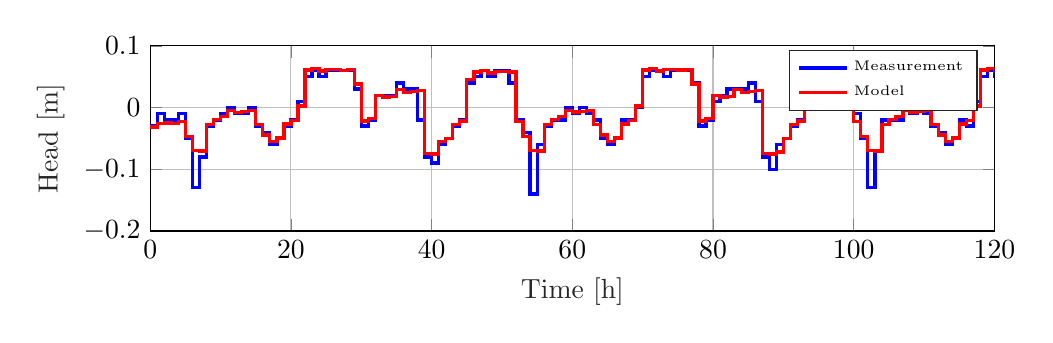
\begin{tikzpicture}

\begin{axis}[%
width=4.221in,
height=0.926in,
at={(0.838in,0.427in)},
scale only axis,
xmin=0,
xmax=120,
grid,
xlabel style={font=\color{white!15!black}},
xlabel={Time [h]},
ymin=-0.2,
ymax=0.1,
ylabel style={font=\color{white!15!black}},
ylabel={Head  [m]},
axis background/.style={fill=white},
title style={},
%title={$\bar{p}_{\mathcal{K},1}$},
legend style={legend cell align=left, align=left, draw=white!15!black}
]
\addplot[const plot, color=blue, line width=1.2pt] table[row sep=crcr] {%
0	-0.0300000000000011\\
1	-0.00999999999999801\\
2	-0.0199999999999996\\
3	-0.0199999999999996\\
4	-0.0100000000000016\\
5	-0.0500000000000007\\
6	-0.129999999999999\\
7	-0.0800000000000018\\
8	-0.0299999999999976\\
9	-0.0199999999999996\\
10	-0.0100000000000016\\
11	0\\
12	-0.0100000000000016\\
13	-0.00999999999999801\\
14	0\\
15	-0.0300000000000011\\
16	-0.0399999999999991\\
17	-0.0599999999999987\\
18	-0.0500000000000007\\
19	-0.0300000000000011\\
20	-0.0199999999999996\\
21	0.0100000000000016\\
22	0.0499999999999972\\
23	0.0600000000000023\\
24	0.0500000000000007\\
25	0.0599999999999987\\
26	0.0599999999999987\\
27	0.0600000000000023\\
28	0.0599999999999987\\
29	0.0300000000000011\\
30	-0.0300000000000011\\
31	-0.0199999999999996\\
32	0.0199999999999996\\
33	0.0199999999999996\\
34	0.0199999999999996\\
35	0.0399999999999991\\
36	0.0300000000000011\\
37	0.0300000000000011\\
38	-0.0199999999999996\\
39	-0.0800000000000018\\
40	-0.0899999999999999\\
41	-0.0599999999999987\\
42	-0.0500000000000007\\
43	-0.0300000000000011\\
44	-0.0199999999999996\\
45	0.0399999999999991\\
46	0.0500000000000007\\
47	0.0600000000000023\\
48	0.0499999999999972\\
49	0.0600000000000023\\
50	0.0599999999999987\\
51	0.0399999999999991\\
52	-0.0199999999999996\\
53	-0.0399999999999991\\
54	-0.140000000000001\\
55	-0.0599999999999987\\
56	-0.0300000000000011\\
57	-0.0199999999999996\\
58	-0.0199999999999996\\
59	0\\
60	-0.0100000000000016\\
61	0\\
62	-0.00999999999999801\\
63	-0.0199999999999996\\
64	-0.0500000000000007\\
65	-0.0599999999999987\\
66	-0.0500000000000007\\
67	-0.0199999999999996\\
68	-0.0200000000000031\\
69	0\\
70	0.0500000000000007\\
71	0.0600000000000023\\
72	0.0599999999999987\\
73	0.0500000000000007\\
74	0.0599999999999987\\
75	0.0600000000000023\\
76	0.0599999999999987\\
77	0.0399999999999991\\
78	-0.0300000000000011\\
79	-0.0199999999999996\\
80	0.0100000000000016\\
81	0.0199999999999996\\
82	0.0300000000000011\\
83	0.0299999999999976\\
84	0.0300000000000011\\
85	0.0399999999999991\\
86	0.0100000000000016\\
87	-0.0800000000000018\\
88	-0.0999999999999979\\
89	-0.0600000000000023\\
90	-0.0499999999999972\\
91	-0.0300000000000011\\
92	-0.0199999999999996\\
93	0.0399999999999991\\
94	0.0500000000000007\\
95	0.0599999999999987\\
96	0.0500000000000007\\
97	0.0599999999999987\\
98	0.0600000000000023\\
99	0.0199999999999996\\
100	-0.0100000000000016\\
101	-0.0500000000000007\\
102	-0.129999999999999\\
103	-0.0700000000000003\\
104	-0.0199999999999996\\
105	-0.0199999999999996\\
106	-0.0199999999999996\\
107	0\\
108	-0.0100000000000016\\
109	0\\
110	-0.00999999999999801\\
111	-0.0300000000000011\\
112	-0.0399999999999991\\
113	-0.0599999999999987\\
114	-0.0500000000000007\\
115	-0.0199999999999996\\
116	-0.0300000000000011\\
117	0.00999999999999801\\
118	0.0500000000000007\\
119	0.0600000000000023\\
120	0.0499999999999972\\
121	0.0600000000000023\\
122	0.0599999999999987\\
123	0.0600000000000023\\
124	0.0599999999999987\\
125	0.0399999999999991\\
126	-0.0300000000000011\\
127	-0.0299999999999976\\
128	0.0199999999999996\\
129	0.0199999999999996\\
130	0.0300000000000011\\
131	0.0299999999999976\\
132	0.0300000000000011\\
133	0.0300000000000011\\
134	0.0199999999999996\\
135	-0.0800000000000018\\
136	-0.0899999999999999\\
137	-0.0700000000000003\\
138	-0.0499999999999972\\
139	-0.0300000000000011\\
140	-0.0199999999999996\\
141	0.0399999999999991\\
142	0.0599999999999987\\
143	0.0500000000000007\\
144	0.0600000000000023\\
145	0.0499999999999972\\
146	0.0600000000000023\\
147	0.0199999999999996\\
};
\addlegendentry{\tiny Measurement}

\addplot[const plot, color=red, line width=1.2pt] table[row sep=crcr] {%
0	-0.0314953408600847\\
1	-0.0261511708145801\\
2	-0.0249388357042098\\
3	-0.0253430790666174\\
4	-0.0228935563842958\\
5	-0.0471330192811219\\
6	-0.0698429798627485\\
7	-0.0704532442880777\\
8	-0.0270647725698969\\
9	-0.0195735077762217\\
10	-0.0149018051780943\\
11	-0.00490460365931585\\
12	-0.00748453068756671\\
13	-0.00641628502194604\\
14	-0.0048269785222319\\
15	-0.0273598720279585\\
16	-0.0445368008891041\\
17	-0.0546615624529683\\
18	-0.0494401514494873\\
19	-0.0267542130421464\\
20	-0.02096241458908\\
21	0.00266197968896239\\
22	0.0605943445324441\\
23	0.06289424675921\\
24	0.0590940417039035\\
25	0.0614627078362112\\
26	0.0615464840202186\\
27	0.0605404962332324\\
28	0.0617067914385518\\
29	0.0379799997152326\\
30	-0.0218592799230074\\
31	-0.0176125388310815\\
32	0.0196388696203121\\
33	0.0169187464667844\\
34	0.0179986311528558\\
35	0.0290458406228877\\
36	0.024559896762181\\
37	0.025651405828004\\
38	0.0277422267830423\\
39	-0.073924844228405\\
40	-0.0753638238111577\\
41	-0.0552469364207819\\
42	-0.0500172645491745\\
43	-0.0274384988209847\\
44	-0.0216542654330567\\
45	0.045873685530065\\
46	0.0574524822163578\\
47	0.0598962622592853\\
48	0.0560745505159747\\
49	0.0585184886228373\\
50	0.0586936066981883\\
51	0.0577036126329718\\
52	-0.0228930353630309\\
53	-0.0471317556480748\\
54	-0.0698425163925433\\
55	-0.070451952573112\\
56	-0.0270257684776636\\
57	-0.0195340349178723\\
58	-0.0148623412749541\\
59	-0.0048269785222319\\
60	-0.00744358189479098\\
61	-0.00633827098381218\\
62	-0.00478809491023346\\
63	-0.0273181938832803\\
64	-0.0444991201976671\\
65	-0.0546195862611518\\
66	-0.049398679816592\\
67	-0.0267109234067873\\
68	-0.020921612718095\\
69	0.00273812501122386\\
70	0.0607736356754975\\
71	0.0631311199777358\\
72	0.0593378889291222\\
73	0.0616913532636117\\
74	0.0617100655013012\\
75	0.0607030164831772\\
76	0.0618630486720332\\
77	0.0382189076834352\\
78	-0.0216603064363593\\
79	-0.017337235679673\\
80	0.0199115688889318\\
81	0.017182921270009\\
82	0.0181816200778616\\
83	0.029280774340784\\
84	0.0247320166292745\\
85	0.0258211744823658\\
86	0.0279065936632696\\
87	-0.0739260697983251\\
88	-0.0753650797776091\\
89	-0.0719189208086672\\
90	-0.0500541111420687\\
91	-0.0274777227456057\\
92	-0.0216939709738741\\
93	0.0457691303179862\\
94	0.0573516330543233\\
95	0.0598001851467871\\
96	0.0559097372376372\\
97	0.0584527682720893\\
98	0.0585396438036973\\
99	0.0575504575739791\\
100	-0.0228927622484217\\
101	-0.0471317556480748\\
102	-0.0698422745773939\\
103	-0.070451952573112\\
104	-0.0270237738780054\\
105	-0.0195340349178723\\
106	-0.0148623412749541\\
107	-0.0048269785222319\\
108	-0.00744358189479098\\
109	-0.00633827098381218\\
110	-0.00478809491023346\\
111	-0.0273181938832803\\
112	-0.0444965052631926\\
113	-0.0546195862611518\\
114	-0.049398679816592\\
115	-0.0267109234067873\\
116	-0.020921612718095\\
117	0.00274046045295254\\
118	0.060842672808763\\
119	0.0631311199777358\\
120	0.0593378889291222\\
121	0.0616953093354183\\
122	0.0617100655013012\\
123	0.0607030164831772\\
124	0.0618630486720332\\
125	0.0382490155772828\\
126	-0.021626292209327\\
127	-0.017337235679673\\
128	0.0199162260341476\\
129	0.017182921270009\\
130	0.0182530633661346\\
131	0.0293107168732958\\
132	0.0247320166292745\\
133	0.0258880536517167\\
134	0.0279390707231862\\
135	-0.0739260697983251\\
136	-0.0753650797776091\\
137	-0.0719194647595778\\
138	-0.0500541111420687\\
139	-0.0274777227456057\\
140	-0.0216939709738741\\
141	0.0457691303179862\\
142	0.0572848480692789\\
143	0.0597970252477602\\
144	0.0559097372376372\\
145	0.0584216984242485\\
146	0.0585396438036973\\
147	0.0575504575739791\\
};
\addlegendentry{\tiny Model}

\end{axis}
\end{tikzpicture}% 
 \vspace{-2.5mm}
 \caption{Validation 2.}
 \label{fig:p_WT_ident_v2}
 \end{figure}

 \vspace{-4mm}

The output parameter vectors $\theta_{\mathcal{K}1}$, $\theta_{\mathcal{K}2}$ and the state parameter vector $\theta_{\mathcal{S}1}$, including the output weights, linear parameters and biases are shown in \eqref{par_matrices_output_example123}.

\vspace{-2mm}

 \begin{equation}
\label{par_matrices_output_example123}
         \theta_{\mathcal{K}1} = 
          \begin{pmatrix}
           -321.27  \\
           -101.81  \\
           -391.47  \\
           -382.66  \\
           -4.48 \cdot 10^6  \\
           4.55 \cdot 10^6 \\
           9.23 \cdot 10^3 \\
           4.48 \cdot 10^6 \\
           394.62 \\
           -4.57 \cdot 10^6\\
           -0.27 \\
           37.33 \\
         \end{pmatrix}
         ,
         \hspace{5mm}
         \theta_{\mathcal{K}2} = 
          \begin{pmatrix}
           -102.36  \\
           10.88  \\
           -89.94  \\
           115.19  \\
           -3.28 \cdot 10^5  \\
           1.42 \cdot 10^5 \\
           -1.78 \cdot 10^3 \\
           3.27 \cdot 10^5 \\
           35.35 \\
           -1.39 \cdot 10^5\\
           -0.33 \\
           60.14 \\
         \end{pmatrix}
\hspace{5mm}
         \theta_{\mathcal{S}1} = 
          \begin{pmatrix}
           4.15 \cdot 10^{3} \\
            2.64 \cdot 10^{4} \\
             -5.15 \cdot 10^{4} \\
              2.51 \cdot 10^{4} \\
               0.42 \\
                -4.15 \cdot 10^{3} \\
                  3.4 \cdot 10^{-3} \\
                   -8.08 \cdot 10^{-4} \\
                   -5.8 \cdot 10^{-3} \\
                    0.16 

         \end{pmatrix}
\end{equation}

\chapter{Test network description}
\label{physical_properties_example1}

\emph{In this part of the appendix, the corresponding physical parameters, control properties and consumption properties are listed for the Multi-inlet, Single-WT example network.}

In order to describe the network, the IDs shown in \figref{fig:epanet_example1_id} and in \figref{fig:epanet_example1_id_pipes} are used to identify the corresponding pipes and measurement points in the network. 

%EPANET example network for identification
\begin{figure}[H]
\centering
%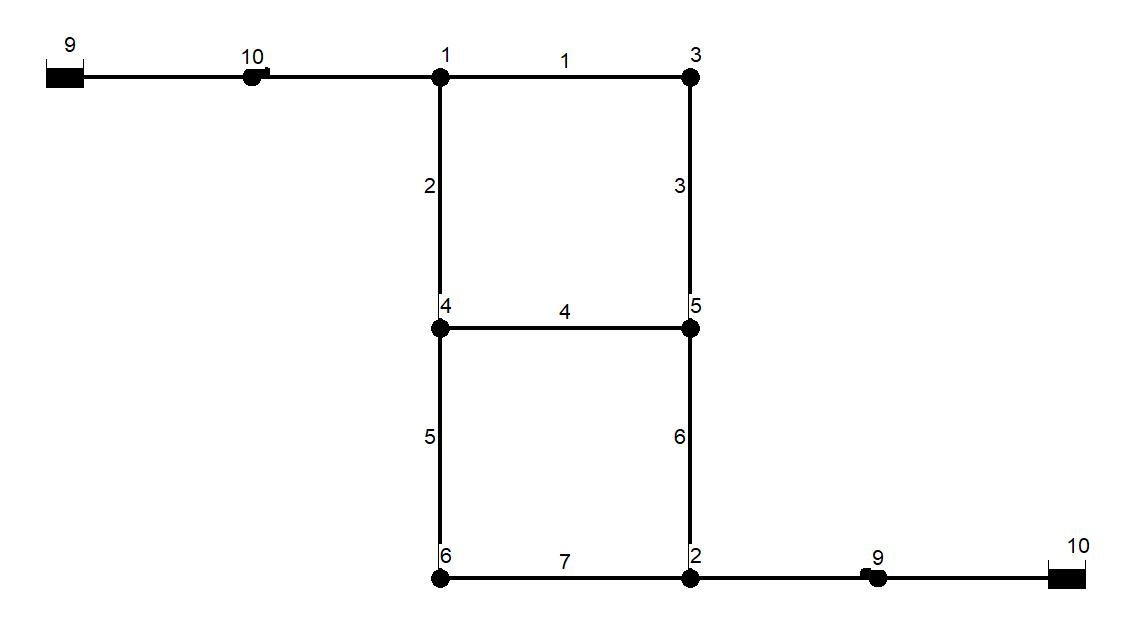
\includegraphics[width=0.6\textwidth]{report/pictures/example1_epanetmodel}
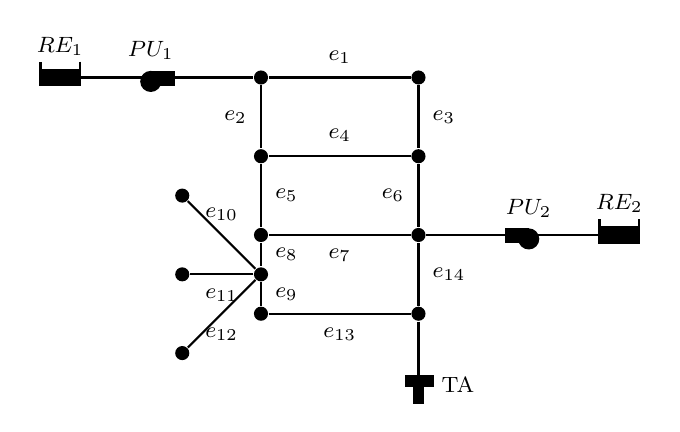
\begin{tikzpicture}[semithick,state/.style ={ draw,shape=circle,scale=0.95}]

\node[circle,fill,inner sep=1.8pt,label=above : \footnotesize$$] (A) at (0,0) {};
\node[circle,fill,inner sep=1.8pt,label=above : \footnotesize$$] (B) at (2,0) {};
\node[circle,fill,inner sep=1.8pt,label= left: \footnotesize$$] (C) at (0,-1) {};
\node[circle,fill,inner sep=1.8pt,label= right: \footnotesize$$] (D) at (2,-1) {};
\node[circle,fill,inner sep=1.8pt,label= above right: \footnotesize $$] (E) at (2,-2) {};
\node[circle,fill,inner sep=1.8pt,label= above left: \footnotesize$$] (F) at (0,-2) {};
\node[circle,fill,inner sep=1.8pt,label= below : \footnotesize$$] (G) at (0,-3) {};
\node[circle,fill,inner sep=1.8pt,label=  right: \footnotesize$$] (H) at (0,-2.5) {};
\node[circle,fill,inner sep=1.8pt,label=  right: \footnotesize$$] (I) at (2,-3) {};
\node[circle,fill,inner sep=1.8pt,label=  above: \footnotesize$$] (J) at (-1,-1.5) {};
\node[circle,fill,inner sep=1.8pt,label=  above: \footnotesize $$] (M) at (-1,-2.5) {};
\node[circle,fill,inner sep=1.8pt,label=  above: \footnotesize $$] (L) at (-1,-3.5) {};



\draw [thick] (A) -- node[above  =0.05 cm] {\footnotesize$e_1$}  (B);
\path (A) edge [thick]  node[left  =0.05 cm] {\footnotesize$e_2$} (C);
\path (B) edge [thick] node[right  =0.05 cm] {\footnotesize$e_3$} (D);
\path (C) edge [thick] node[above  =0.05 cm] {\footnotesize$e_4$} (D);
\path (C) edge [thick] node[right  =0.05 cm] {\footnotesize$e_5$} (F);
\path (D) edge [thick] node[left  =0.05 cm] {\footnotesize$e_6$} (E);
\path (E) edge [thick] node[below  =0.05 cm] {\footnotesize$e_7$} (F);
\path (F) edge [thick] node[right  =0.05 cm] {\footnotesize$e_8$} (H);
\path (H) edge [thick] node[right  =0.05 cm] {\footnotesize$e_9$} (G);
\path (H) edge [thick] node[above  =0.05 cm] {\footnotesize$e_{10}$} (J);
\path (H) edge [thick] node[below  =0.05 cm] {\footnotesize$e_{11}$} (M);
\path (H) edge [thick] node[below  =0.05 cm] {\footnotesize$e_{12}$} (L);
\path (G) edge [thick] node[below  =0.05 cm] {\footnotesize$e_{13}$} (I);
\path (E) edge [thick] node[right  =0.05 cm] {\footnotesize$e_{14}$} (I);

%PU2
\node[circle,fill,inner sep=2.7pt,label= above : \footnotesize $ PU_2$] (I) at (3.4,-2.05) {};
\draw [thin,fill] (3.1,-1.92) rectangle (3.4,-2.1);


\begin{scope}[xscale=-1,yscale=1]
%PU1
\node[circle,fill,inner sep=2.7pt,label= above : \footnotesize $ PU_1$] (I) at (3.4-2,-2.05+2) {};
\draw [thin,fill] (3.1-2,-1.92+2) rectangle (3.4-2,-2.1+2);

\end{scope}

\draw [thick](2.1,-2) -- (3.1,-2);
\draw [thick, fill] (1.84,-3.79) rectangle (2.18,-3.92);
\draw [thick,fill] (1.95,-3.92) rectangle (2.06,-4.13);
\draw [thick](2,-3.1) -- (2,-3.8);
\node at (2.5,-3.9) {\footnotesize TA};


\draw [thick](-0.1,0) -- (-1.1,0);


\draw [thick](3.5,-2) -- (4.3,-2);
\draw [thick](-1.5,0) -- (-2.3,0);
\draw [thick](-2.3,0.2) -- (-2.3,-0.1) -- (-2.8,-0.1) -- (-2.8,0.2);
\draw [thick,fill] (-2.8,0.1) rectangle (-2.3,-0.1);
\draw [thick](4.3,-1.8) -- (4.3,-2.1) -- (4.8,-2.1) -- (4.8,-1.8);
\draw [thick,fill] (4.3,-1.9) rectangle (4.8,-2.1);
\node at (-2.55,0.4) {\footnotesize $RE_1$};
\node at (4.55,-1.6) {\footnotesize $RE_2$};
\end{tikzpicture} 
\caption{Pipe IDs in the test network.}
\label{fig:epanet_example1_id_pipes}
\end{figure}
\vspace{-3mm}

The physical properties of pipes are shown in \tabref{pipes_table_example1}.

\vspace{-3mm}

\begin{center}
    \begin{tabular}{ | >{\centering\arraybackslash}m{1.8cm} | >{\centering\arraybackslash}m{3.6cm} | >{\centering\arraybackslash}m{3.6cm} | >{\centering\arraybackslash}m{3.6cm} |}
    \hline
    \multirow{1}{*}
     Pipe ID & Length, l[m] & Diameter, D[mm] & Roughness, $\epsilon$[mm] \\ 
     \hline
     \multirow{1}{*}
    \text{$e_1$} & 350 & 200 & 50 \\ 
    \hline
      \multirow{1}{*}
    \text{$e_2$} & 500 & 200  & 150 \\ 
    \hline
      \multirow{1}{*}
    \text{$e_3$} & 500 & 200 & 30 \\ 
    \hline
      \multirow{1}{*}
    \text{$e_4$} & 350 & 200 & 50 \\ 
    \hline
    \multirow{1}{*}
    \text{$e_5$} & 500 & 200 & 30 \\ 
    \hline
    \multirow{1}{*}
    \text{$e_6$} & 500 & 200 & 10 \\ 
    \hline
    \multirow{1}{*}
    \text{$e_7$} & 350 & 200 & 10 \\ 
    \hline
    \multirow{1}{*}
    \text{$e_8$} & 350 & 200 & 0.005 \\ 
    \hline
    \multirow{1}{*}
    \text{$e_9$} & 350 & 200 & 0.005 \\ 
    \hline
    \multirow{1}{*}
    \text{$e_{10}$} & 350 & 200 & 0.005 \\ 
    \hline
    \multirow{1}{*}
    \text{$e_{11}$} & 350 & 200 & 10 \\ 
    \hline
    \multirow{1}{*}
    \text{$e_{12}$} & 350 & 200 & 50 \\ 
    \hline
    \multirow{1}{*}
    \text{$e_{13}$} & 350 & 200 & 50 \\ 
    \hline
    \multirow{1}{*}
    \text{$e_{14}$} & 350 & 200 & 1 \\ 
    \hline
    \multirow{1}{*}
    \text{$e_{15}$} & 350 & 200 & 0.005 \\ 
    \hline
    \end{tabular}
    \captionof{table}{Physical properties of pipes in the test network.}
    \label{pipes_table_example1}
\end{center}

The pumping stations $PU_1$ and $PU_2$ are described by \eqref{pu1_pumpcurve} and \eqref{pu2_pumpcurve} pump curves, respectively. 


\begin{subequations}

\begin{equation}
\label{pu1_pumpcurve}
h = 53.33 - 0.008334 q^2, 
\end{equation}

\vspace{-2mm}

\begin{equation}
\label{pu2_pumpcurve}
h = 46.67 - 0.009525 q^2. 
\end{equation}

\end{subequations}

Furthermore, the elevation of the WT is 21 meters, the initial level is 19.5 meters, the minimum level is 2 meters and the maximum level is 21 meters. The diameter of the WT is 50 meters. 

The physical properties of the nodes are shown in \tabref{pipes_table_example1_nodes}.

\begin{center}
    \begin{tabular}{ | >{\centering\arraybackslash}m{1.8cm} | >{\centering\arraybackslash}m{3.6cm} | >{\centering\arraybackslash}m{3.6cm} | }
    \hline
    \multirow{1}{*}
     Node ID & Elevation, h[m] & Diameter, D[m]  \\ 
     \hline
     \multirow{1}{*}
    \text{$n_1$} & 0 & 0 \\ 
    \hline
      \multirow{1}{*}
    \text{$n_2$} & 2 & 5   \\ 
    \hline
      \multirow{1}{*}
    \text{$n_3$} & 0 & 0 \\ 
    \hline
      \multirow{1}{*}
    \text{$n_4$} & 0 & 0  \\ 
    \hline
    \multirow{1}{*}
    \text{$n_5$} & 20 & 15 \\ 
    \hline
    \multirow{1}{*}
    \text{$n_6$} & 0 & 5 \\ 
    \hline
    \multirow{1}{*}
    \text{$n_7$} & 0 & 5  \\ 
    \hline
    \multirow{1}{*}
    \text{$n_8$} & 0 & 5  \\ 
    \hline
    \multirow{1}{*}
    \text{$n_9$} & 0 & 0  \\ 
    \hline
    \multirow{1}{*}
    \text{$n_{10}$} & 0 & 0  \\ 
    \hline
    \multirow{1}{*}
    \text{$n_{11}$} & 0 & 0 \\ 
    \hline
    \multirow{1}{*}
    \text{$n_{12}$} & 0 & 0 \\ 
    \hline
    \end{tabular}
    \captionof{table}{Physical properties of nodes in the test network.}
    \label{pipes_table_example1_nodes}
\end{center}